%==============================================================================
% DRAFT -- single-file working copy.   Compile:  tectonic draft.tex
%
% >>> THIS FILE IS THE LIVE COPY. Edit here. <<<
% chapters/*.tex and main.tex are FROZEN and now out of date. Do not edit them
% until the split-back below has happened.
%
% SPLIT-BACK PLAN (when the official EPCC template arrives / drafting settles):
%   Each chapter is preceded by a  "% ===== FILE: chapters/xxx.tex ====="  marker.
%   Cut at those markers into the matching files under chapters/, drop this
%   preamble (main.tex already has it), and main.tex compiles unchanged.
%   Keep \chapter/\section as-is: the structure is already the dissertation's.
%
% Draft settings: `oneside` = no blank pages between chapters. The printed
% submission uses [11pt,a4paper,twoside,openright] + geometry bindingoffset=6mm.
%==============================================================================
\documentclass[11pt,a4paper,oneside]{report}

%------------------------------------------------------------------ engine-safe fonts
\usepackage{iftex}
\ifPDFTeX
  \usepackage[utf8]{inputenc}
  \usepackage[T1]{fontenc}
  \usepackage{lmodern}
\else
  \usepackage{fontspec}
\fi

%------------------------------------------------------------------ layout & graphics
\usepackage[a4paper,margin=2.5cm]{geometry}
\usepackage{graphicx}
% figures/ ONLY. Never point this at the analysis/ tree: reorganising the plots
% directory then silently breaks the build. Refresh with ./sync_figures.sh.
\graphicspath{{figures/}}
\usepackage{booktabs}
% array: ragged-right p columns, so the long paths in the evidence index wrap
% without stretching the inter-word space past the column edge.
\usepackage{array}
\newcolumntype{L}[1]{>{\raggedright\arraybackslash}p{#1}}
\usepackage{amsmath,amssymb}
\usepackage{listings}
\usepackage{microtype}
\usepackage{csquotes}

%------------------------------------------------------------------ bibliography
\usepackage[backend=biber,style=numeric-comp,sorting=none]{biblatex}
\addbibresource{references.bib}

%------------------------------------------------------------------ links (load late)
\usepackage[hidelinks]{hyperref}
\usepackage[capitalise]{cleveref}

\emergencystretch=2em

\title{Hybrid MPI+OpenMP Performance of PETSc Krylov Solvers on ARCHER2}
\author{Leyan Li}
\date{August 2026}

\begin{document}

% ===== FILE: chapters/00_frontmatter.tex =====
\pagenumbering{roman}
\hypersetup{pageanchor=false}
\begin{titlepage}
\centering
\vspace*{2cm}
{\LARGE\bfseries Hybrid MPI+OpenMP Performance of PETSc\\[0.3em]
Krylov Solvers on ARCHER2\par}
\vspace{2cm}
{\Large Leyan Li\par}
\vspace{1cm}
{\large MSc in High Performance Computing\par}
{\large EPCC, University of Edinburgh\par}
\vspace{1cm}
{\large August 2026\par}
\vfill
{\normalsize A dissertation submitted in partial fulfilment\\
of the requirements for the degree of\\
Master of Science.\par}
\end{titlepage}
\hypersetup{pageanchor=true}
\clearpage

\chapter*{Abstract}
\addcontentsline{toc}{chapter}{Abstract}
PETSc can combine MPI ranks with OpenMP threads, but the best balance depends on solver
work, communication, and the decomposition. This dissertation measures four full-node
layouts on ARCHER2: 128 MPI ranks with one thread per rank, and hybrid layouts with two,
four, or eight threads per rank. Matched two- and three-dimensional Poisson benchmarks
cover six problem sizes from 5.0 to 164.6 million unknowns on 1--32 nodes. Each formal
configuration has three runs. One warm-up solve builds the GAMG hierarchy; 19 timed solves
then reuse it in a dedicated PETSc logging stage. The unknowns-per-core admission filter
orders the 11 admitted size--node pairs into two weak-scaling chains, along which the
layout comparison is made at constant work per core.

The two dimensions differ in the shape of the result, not only in which layout is fastest.
In 2D the layout effect is ordered by concurrency: every hybrid layout improves relative
to flat MPI as the node count grows, monotonically in four of the six measured series.
$64\times2$ is faster per iteration than flat MPI at all 11 pairs, by 4.3\% at one node
and 12.8\% at 16, and reaches 13.1\% higher raw throughput at 164.56 million unknowns on
32 nodes; $32\times4$ crosses from 9.6\% slower at one node to 6.3\% faster at 32. In 3D
the advantage is larger, reaching 33.2\%, but no series is monotone and the preferred
layout changes with scale and node count. Eight threads per rank wins no point in either
dimension at constant work per core.

A matched extension holds the problem size fixed near 20 million unknowns and scales from
one to 32 nodes, and there the layouts differ in where they saturate rather than only in
speed. The 2D curves stay within a factor of 1.81 of each other and all four are still improving
at 4096 cores, whereas in 3D every layout saturates and turns upward at a node count that
rises with its thread count: eight nodes for flat MPI, which is $2.6\times$ slower again
by 32, and beyond 32 for $16\times8$, which ends $3.81\times$ faster than it. What
distinguishes the
layouts under strong scaling is where they stop scaling, so the same layout is both the
worst choice at comfortable occupancy and the best one past saturation. PETSc event data
show hybridisation reducing exposure to halo exchange and global reduction, and eleven
Linaro MAP profiles measure the cost that repays: the share of core-time spent waiting in
the OpenMP runtime rises with threads per rank, reproducibly across two builds, and the
linked threaded BLAS library accounts for at most 2.1\% of solve-window core-time. The
hardware mechanism behind the waiting is not established here.

\chapter*{Acknowledgements}
\addcontentsline{toc}{chapter}{Acknowledgements}
% TODO: supervisor, EPCC, ARCHER2 access.

\tableofcontents
\listoffigures
\listoftables
\clearpage

\pagenumbering{arabic}

% ===== FILE: chapters/ch1_introduction.tex =====
\chapter{Introduction}
\label{ch:intro}
% Rewritten 2026-07-31, once the results were final. RQ1-RQ4 follow the feasibility study
% §4.1, narrowed to what the completed campaigns can actually answer.

\section{Motivation}
\label{sec:motivation}
Sparse iterative solvers dominate the run time of a large class of scientific applications,
and PETSc \cite{petsc_manual_324,petsc1997} is one of the most widely used libraries for
writing them. PETSc has always parallelised across distributed memory with MPI. Since
version 3.22 it can also be configured with threaded kernels, so a fixed allocation of
cores can be spent on MPI ranks, on OpenMP threads inside each rank, or on any combination
of the two \cite{petsc_openmp_backend}.

That choice is not obviously free. An ARCHER2 compute node provides 128 physical cores
across two sockets, eight NUMA regions, and thirty-two four-core shared-L3 domains. Flat
MPI exposes every subdomain as a separate process with its own address space, message
matching, and solver metadata. Replacing ranks with threads reduces the number of MPI
endpoints and of subdomain boundaries, but requires the runtime to create, schedule, and
synchronise thread teams, and makes several cores compete for the same caches and memory
channels. Both effects grow with the thread count, in opposite directions.

Neither effect can be predicted from the core count. The saving depends on how much of an
iteration is actually spent communicating, which depends in turn on the problem size, the
stencil, the preconditioner, and the number of nodes; the cost depends on how much work
each threaded kernel exposes and on where the threads sit in the memory hierarchy. A user
allocating a full ARCHER2 node has four sensible layouts available and no principled way to
choose between them. The purpose of this dissertation is to measure that choice.

\section{Aims and Research Questions}
\label{sec:aims}
This study measures PETSc rank--thread configurations for matched two- and
three-dimensional Poisson problems on ARCHER2. It compares flat MPI with three hybrid
MPI+OpenMP layouts across six problem sizes from 5.0 to 164.6 million unknowns and 1--32
fully populated nodes, holding the core count, the solver, and the convergence criteria
fixed so that only the layout varies. Because the admission rule that keeps the work per
core constant also limits each problem size to one or two node counts, a matched extension
repeats the same contract on a fixed problem of about 20 million unknowns over the whole
node range, so that the two standard scaling regimes are both covered. Four questions
follow the feasibility study that preceded this work, narrowed to what the completed
campaigns can answer.

\begin{description}
  \item[RQ1] Does PETSc's threaded-kernel backend reduce the time to solution relative to
    flat MPI on a fully populated node, and by how much?
  \item[RQ2] If it does, at which rank--thread balances, and how does the answer change
    with problem size, node count, dimensionality, and scaling regime?
  \item[RQ3] Which parts of the solve account for the difference?
  \item[RQ4] How far do the observed trends generalise, and what would be needed to
    establish a mechanism for them?
\end{description}

RQ1 and RQ2 are answered by \Cref{ch:multinode}, RQ3 by \Cref{ch:profiling}, and RQ4 by
\Cref{ch:discussion}. The feasibility study's hypotheses expected a benefit at two to four
threads per rank and expected \texttt{VecMDot} and \texttt{PCApply} to be the limiting
kernels. The first expectation is borne out. The second was formed while the study still
used PETSc's default GMRES solver; the change of solver described in \Cref{sec:solver}
replaces \texttt{VecMDot} with \texttt{VecTDot} and moves the dominant cost elsewhere.

\section{Contributions}
\label{sec:contributions}
\begin{enumerate}
  \item \textbf{A matched 2D and 3D rank--thread study at full node occupancy.} Four
    layouts, six problem sizes, 1--32 nodes, three formal repeats, and 264 content-validated
    formal runs, with a further 144 runs on matched fixed-size problems. Every log is
    checked against the intended build, the requested rank and thread counts, the expected
    number of converged solves, and the linked library, and the parsed results are
    reconciled against the independently retrieved job CSVs.

  \item \textbf{Evidence that the layout ranking depends on concurrency, not just on the
    workload.} Read as weak scaling at fixed unknowns per core, the 2D advantage of
    hybrid execution grows monotonically with node count: $64\times2$ is faster per
    iteration than flat MPI at all 11 size--node points, by 4.3\% at one node and 12.8\% at
    16, and $32\times4$ crosses from 9.6\% slower at one node to 6.3\% faster at 32. A
    layout comparison performed at small node counts does not transfer to large ones.

  \item \textbf{Evidence that the layout ranking also depends on the scaling regime.} On
    matched fixed-size problems near 20 million unknowns, scaled from one to 32 nodes, the
    2D layouts remain within a factor of 1.81 of each other and all keep scaling, while the
    3D layouts diverge to a factor of 3.81 because each saturates and turns upward at a node
    count that rises with its thread count --- eight nodes for flat MPI, 16 for the two
    intermediate layouts, and beyond 32 for $16\times8$. $16\times8$ is last at constant work
    per core and first at 4096 cores on a fixed problem, so the same measurement supports
    opposite advice in the two regimes.

  \item \textbf{A quantitative account of why, from both sides of the trade.} PETSc's own
    event data show that hybridisation reduces the share of the solve exposed to halo
    exchange and global reduction at 21 of 22 size--node points, and that within each layout
    the size of that reduction correlates with the speed advantage. Eleven Linaro MAP
    profiles, parsed directly from the profile files, measure the countervailing cost as
    time spent waiting in the OpenMP runtime, which rises with threads per rank while the
    MPI share falls, reproducibly across two PETSc builds. Each doubling of threads per rank
    removes more exposure but must remove more before it repays that cost, which explains
    the two-to-four-thread optimum, the non-monotone 3D ordering, and why $16\times8$ is
    slowest in 2D despite removing the most exposure.

  \item \textbf{A repeated-solve measurement method.} A driver that pays the GAMG setup once
    and then times 19 solves in a dedicated PETSc logging stage, so the reported figures are
    steady-state solve costs rather than a mixture of hierarchy construction and solve. The
    same design is used for the scaling results and for the profiling analysis.

  \item \textbf{A reproducible pipeline and an explicit account of what the evidence does
    not support.} Raw logs, analysis scripts, and figure generation are version-controlled
    and re-runnable from one command per campaign, including the profiler analysis, which
    is computed from the MAP files themselves rather than from a GUI export.
    \Cref{sec:threats} states the limits, including why a rank-dependent preconditioner and
    a silently ignored tolerance option together make the earlier default-solver comparison
    ill-posed, and why no hardware mechanism is claimed.
\end{enumerate}

\section{Dissertation Structure}
\label{sec:structure}
\Cref{ch:background} introduces the execution models, the ARCHER2 node hierarchy, CG with
algebraic multigrid, and the two profiling tools, and identifies the gap this work
addresses. \Cref{ch:methodology} defines the drivers, the solver configuration and why it
was changed, the admissible configuration space, thread placement, and the metrics.
\Cref{ch:multinode} presents the validated 2D and 3D results as weak scaling along two
unknowns-per-core chains, then as fixed-size strong scaling from one to 32 nodes.
\Cref{ch:profiling} explains the measurement design and gives the profiler and
event-level bottleneck analysis. \Cref{ch:discussion} answers the research questions, states
the threats to validity, and gives practical guidance, before \Cref{ch:conclusion}
summarises the findings and the work that remains.

% ===== FILE: chapters/ch2_background.tex =====
\chapter{Background and Related Work}
\label{ch:background}

\section{Parallel Programming Models}
\label{sec:models}
PETSc applications run on machines whose memory is distributed across nodes and
non-uniform within each node. The programming model determines which of these boundaries
the application exposes explicitly.

MPI uses independent processes with private address spaces. Processes exchange data
through point-to-point operations and collectives defined by the MPI standard
\cite{mpi41}. This model matches a distributed-memory machine: each rank owns part of the
problem, and communication makes remote dependencies explicit. MPI implementations also
run within a node, often through shared-memory transports, so ``MPI-only'' does not imply
that every message crosses the network. It does retain process-level decomposition,
message matching, and per-rank library state.

OpenMP uses a shared-memory, fork--join execution model. Threads in a team can access the
same address space, while worksharing constructs divide loop iterations among them
\cite{openmp52}. OpenMP removes the need to express intra-process data exchange as
messages, but the runtime must create or wake thread teams, distribute work, and
synchronise them. Threads can also contend for cache capacity and memory bandwidth. A
threaded loop is therefore faster only when it exposes enough work to offset these costs.

A hybrid program assigns one or more MPI ranks to each node and creates an OpenMP team
inside every rank. MPI still communicates between subdomains; OpenMP processes the data
owned by each rank. The rank--thread product gives the number of cores used, but two
layouts with the same product are not equivalent. For example, $128\times1$ creates 128
subdomains and MPI endpoints on an ARCHER2 node, whereas $32\times4$ creates 32 larger
subdomains and four threads per subdomain. The latter can reduce rank-local metadata and
the number of halo interfaces, but adds thread scheduling and shared-resource contention.
\Cref{tab:models} summarises what each model makes explicit and what it therefore costs.

\begin{table}[ht]
  \centering
  \caption{The three execution models as they apply within one ARCHER2 node. The hybrid
  row is the subject of this dissertation; it inherits both cost columns.}
  \label{tab:models}
  \begin{tabular}{l p{0.20\textwidth} p{0.21\textwidth} p{0.34\textwidth}}
    \toprule
    Model & Memory & Data exchange & Principal cost \\
    \midrule
    MPI    & Private per rank
           & Explicit messages
           & Message matching, per-rank solver state, one subdomain boundary per rank \\
    \addlinespace
    OpenMP & Shared within a team
           & Shared addresses
           & Team creation, synchronisation, cache and bandwidth contention \\
    \addlinespace
    Hybrid & Shared inside a rank, private between ranks
           & Messages between ranks only
           & Both, traded against each other by the rank--thread balance \\
    \bottomrule
  \end{tabular}
\end{table}

Partitioned Global Address Space models such as OpenSHMEM and Chapel express locality
differently again, but PETSc uses MPI for distributed-memory communication, so the
comparison here is between flat MPI and PETSc's hybrid path rather than between
programming-model families.

\section{Limitations of Flat MPI}
\label{sec:flatmpi}
Flat MPI assigns one rank to each core. Its main advantage is uniformity: the same domain
decomposition and communication model applies within and between nodes, and each rank
executes single-threaded code. This often gives predictable performance and avoids thread
safety and OpenMP scheduling costs. A hybrid configuration must outperform this strong
baseline, not an abstract MPI implementation.

The costs of flat MPI become visible under either of the two standard scaling regimes, and
this dissertation uses both, so the distinction is worth stating precisely. Under
\emph{strong} scaling the global problem size is fixed while the core count grows, so the
work per core falls. Under \emph{weak} scaling the problem size grows with the core count
so that the work per core stays constant, and perfect weak scaling would hold the time per
iteration constant. Strong scaling measures how far a fixed problem can be spread; weak
scaling measures what concurrency costs once the local work is held still. The unknowns-
per-core admission rule in \Cref{sec:configspace} makes the second regime the natural
reading of the campaign, and \Cref{sec:bands} sets it out.

Under strong scaling, each rank receives less local work, but latency-sensitive operations
do not shrink at the same rate. A stencil matrix-vector product still exchanges boundary
values, and Krylov dot products still require collective reductions. As the local subdomain
contracts, its boundary-to-interior ratio grows and communication occupies a larger share
of an iteration. More ranks also increase the number of subdomains and may replicate solver
or preconditioner metadata.

Weak scaling does not remove these costs, it isolates them. Holding the unknowns per core
fixed keeps the local kernel work per iteration roughly constant, so any growth in the time
per iteration is attributable to concurrency: more neighbours to exchange with, more ranks
participating in each global reduction, and a longer reduction tree. That is why a weak-
scaling curve is the appropriate place to look for the effect of replacing MPI ranks with
OpenMP threads, and why \Cref{ch:multinode} reports the campaign that way.

Replacing ranks with threads changes these costs rather than removing them. Larger
rank-local subdomains can reduce MPI endpoints and aggregate messages, while threads work
on data already inside the process. Judge's ARCHER2 study found that two or four threads
per rank often improved CP2K and CASTEP, whose runs contained expensive collective
communication, but brought little benefit to the tested molecular-dynamics cases until
their scaling limits \cite{judge2022mpiopenmp}. The relevant conclusion is
application-specific: hybrid execution helps when the saved MPI and memory costs exceed
the added thread overhead.

\section{Hybrid MPI+OpenMP}
\label{sec:hybrid}
Hybrid performance depends on three coupled choices: the number of ranks, the number of
threads in each rank, and their placement on the node. Increasing the thread count reduces
the rank count at fixed cores, but gives each OpenMP region more threads to coordinate.
Sparse linear algebra is a demanding case because its indirect memory accesses and low
arithmetic intensity can saturate memory bandwidth before all cores are busy.

Lange et al. demonstrated that PETSc sparse matrix-vector multiplication could strong
scale beyond a pure-MPI limit by combining MPI with task-based OpenMP, explicit
communication overlap, and thread load balancing \cite{lange_petsc_hybrid}. Their result
establishes that hybrid PETSc execution can work, but it does not predict the performance
of the current PETSc backend. Their implementation targeted a specific matrix kernel and
required optimisations beyond changing the number of threads.

PETSc 3.22 added the configure option \texttt{--with-openmp-kernels}
\cite{petsc_openmp_backend}. This option enables OpenMP in kernels that PETSc has
annotated for threaded execution; it does not replace PETSc's MPI decomposition or make
every solver phase threaded. The build studied here uses both
\texttt{--with-openmp=1} and \texttt{--with-openmp-kernels=1}. A run with one thread per
rank uses the same binary as a hybrid run, which isolates the runtime layout from compiler
and library differences.

This distinction is important for interpreting a negative result. Weak hybrid scaling can
come from a kernel with too little work per thread, a serial or MPI-dominated phase, poor
placement, or shared-memory contention. Runtime alone cannot distinguish these causes;
the profiling method in \Cref{sec:tools} is needed to locate them.

\section{ARCHER2 Node Architecture and NUMA}
\label{sec:archer2}
An ARCHER2 compute node contains two 64-core AMD EPYC 7742 (Rome) processors, giving 128
physical cores. The service configures four NUMA regions per socket, eight per node, with
16 cores and local memory channels in each region. A core has private L1 and L2 caches.
Four cores form a Core Complex (CCX) and share 16\,MB of L3; two CCXs form a Core Complex
Die (CCD). Different CCXs do not share L3 \cite{archer2_hardware}.

This topology is not taken from documentation alone. It was confirmed on an ARCHER2
compute node by a dedicated diagnostic job, because the whole interpretation of the
$16\times8$ layout depends on where the boundaries actually fall. \texttt{lscpu} reports
two sockets of 64 cores, 256 logical CPUs with simultaneous multithreading enabled in
hardware, eight NUMA nodes, and 512\,MiB of L3 in 32 instances, that is 16\,MiB per
instance. \texttt{numactl} shows each NUMA node holding exactly 16 physical cores and
roughly 32\,GB of memory, with relative distances of 10 within a region, 12 between
regions on the same socket, and 32 across the sockets. The sysfs cache topology gives each
L3 instance a \texttt{shared\_cpu\_list} of exactly four physical cores, and
\texttt{hwloc-ls} shows the same 16\,MB L3 above four cores. Every layout in this study is
therefore placed against measured boundaries of four cores per L3 and 16 cores per NUMA
region.
% G11 CLOSED 2026-08-01 from scripts/ksp/diagnostics/petsc_diagnostics.14598711.out
%   (sections G11-a..d). lscpu: 2 sockets x 64 cores, 256 CPUs, SMT 2, L3 512 MiB in 32
%   instances (= 16 MiB each), 8 NUMA nodes of 16 cores (node0 0-15,128-143). numactl
%   distances 10/12/32. sysfs index3 shared_cpu_list = "0-3,128-131" etc., i.e. 4 physical
%   cores per L3. hwloc-ls: "L3 L#0 (16MB)" above four Core objects. The runs themselves
%   use --hint=nomultithread, so the 128 physical cores are used and the SMT siblings idle.

\begin{figure}[htbp]
  \centering
  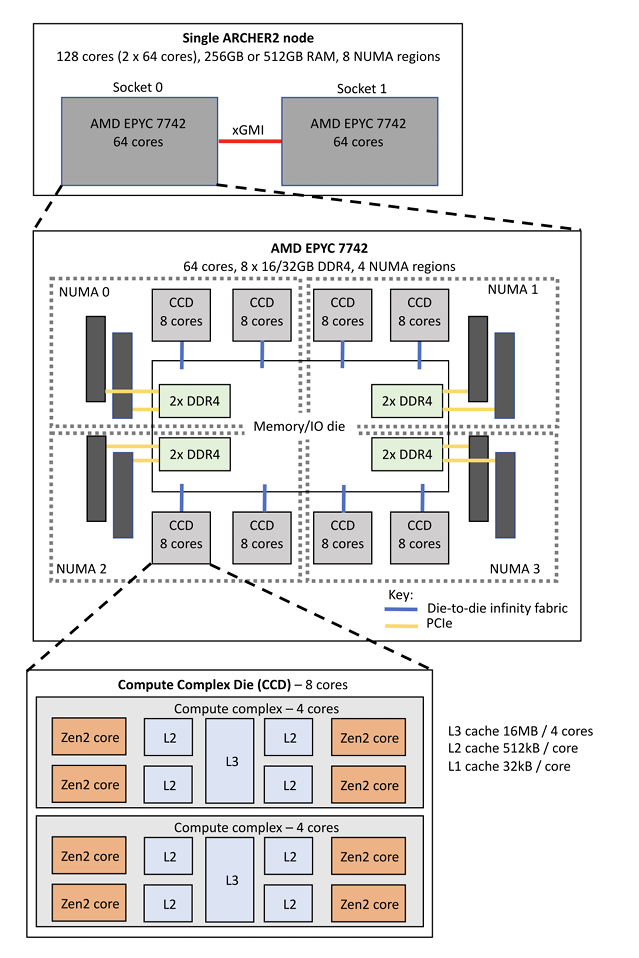
\includegraphics[width=0.58\textwidth]{archer2.png}
  \caption{Hierarchy of an ARCHER2 compute node. Each node has two 64-core AMD EPYC
  7742 processors, eight 16-core NUMA regions, and four-core CCXs that each share
  16\,MB of L3 cache. Source: ARCHER2 hardware documentation
  \cite{archer2_hardware}.}
  \label{fig:archer2_architecture}
\end{figure}

NUMA affects both latency and bandwidth. Linux normally allocates a page in the NUMA
region of the thread that first writes it. If one thread initialises a large array and a
team later accesses it from several regions, remote traffic can concentrate on the memory
controllers of the first region. The ARCHER2 tuning guide also notes that two threads can
approach the memory-bandwidth limit of a NUMA region for bandwidth-intensive code
\cite{archer2_tuning}. More threads do not guarantee more bandwidth.

Cache topology introduces a finer boundary than NUMA: four adjacent cores share an L3
cache, whereas a 16-core NUMA region contains four such L3 domains. With the close binding
of \Cref{sec:placement}, the four full-node layouts therefore sit differently in the
hierarchy, as \Cref{tab:layouts} sets out.

\begin{table}[ht]
  \centering
  \caption{The four fully populated layouts against the ARCHER2 node hierarchy, with
  close binding. Every layout uses all 128 physical cores; what changes is the number of
  subdomains and where each rank's threads sit relative to the shared-L3 and NUMA
  boundaries. The counts are arithmetic from the node topology measured above; they
  describe placement, not a measured claim about cause.}
  \label{tab:layouts}
  \begin{tabular}{lrrl}
    \toprule
    Layout & Cores/rank & Subdomains/node & Rank against the shared-L3 (CCX) boundary \\
    \midrule
    $128\times1$ & 1 & 128 & four ranks share one CCX \\
    $64\times2$  & 2 &  64 & two ranks share one CCX \\
    $32\times4$  & 4 &  32 & exactly one CCX \\
    $16\times8$  & 8 &  16 & spans two CCXs \\
    \bottomrule
  \end{tabular}
\end{table}

The last row is the one to read carefully. A rank of eight threads crosses the shared-L3
boundary, because a CCX is four cores, but it still fits inside a single 16-core NUMA
region: none of the four layouts makes a rank span two NUMA regions. Any account of why
$16\times8$ behaves differently must therefore appeal to L3 capacity or to OpenMP cost, not
to NUMA placement. This mapping is a plausible mechanism for layout differences, not proof
of their cause; the experiments fix thread affinity and compare measurements before using
topology to interpret the ordering. \Cref{sec:map-matrix} returns to it with profiler
evidence and finds that the cost which distinguishes $16\times8$ is paid in the OpenMP
runtime rather than at either memory boundary.

\section{PETSc and Krylov Solvers}
\label{sec:petsc-krylov}
PETSc provides distributed vectors and matrices, Krylov subspace solvers (KSP),
preconditioners (PC), and the logging infrastructure used in this study. PETSc uses MPI
for its distributed-memory communication and lets users select solver components at run
time \cite{petsc_manual_324,petsc1997}. This composition is useful for experiments, but it
also means that a comparison of parallel layouts is meaningful only when the numerical
method performs comparable work in every layout.

The production system is the finite-difference Laplacian, whose matrix is sparse,
symmetric, and positive definite. Conjugate gradients (CG) is designed for this class of
linear system \cite{hestenes1952cg}. At each iteration CG applies the matrix and the
preconditioner, updates vectors, and evaluates inner products. These operations expose two
different scaling limits, and the distinction runs through the whole dissertation: the
sparse matrix-vector product exchanges halo values with \emph{neighbouring} subdomains,
whereas inner products and residual norms require a reduction across \emph{all} ranks.
\Cref{tab:cg-ops} classifies the work of one iteration accordingly.

\begin{table}[ht]
  \centering
  \caption{Operations in one GAMG-preconditioned CG iteration, with the PETSc event that
  records each and the number of calls per outer iteration measured in a representative
  run. Neighbour and global costs scale differently with the rank count, which is why
  \Cref{sec:bottleneck} separates them.}
  \label{tab:cg-ops}
  \begin{tabular}{lllr}
    \toprule
    Operation & PETSc event & Communication & Calls \\
    \midrule
    Matrix-vector product   & \texttt{MatMult}          & neighbour &  28.9 \\
    Multigrid restriction   & \texttt{MatMultTranspose} & neighbour &   7.0 \\
    Multigrid prolongation  & \texttt{MatMultAdd}       & neighbour &   7.0 \\
    Level residual          & \texttt{MatResidual}      & neighbour &   7.0 \\
    \addlinespace
    Halo exchange, all of the above & \texttt{VecScatterBegin} & neighbour & 42.9 \\
    \addlinespace
    Inner products          & \texttt{VecTDot}          & global    &   2.0 \\
    Residual norm           & \texttt{VecNorm}          & global    &   1.0 \\
    Vector updates          & \texttt{VecAXPY}, \texttt{VecAYPX} & none & 44.6 \\
    \bottomrule
  \end{tabular}
\end{table}
% VERIFIED 2026-07-31 from analysis/data/nproc_2d_libsci/logs/repeated_fullnode/165m/
%   nodes16/logs/ex2_..._ppn128_t1_job14528993_rep1.log: RepeatedSolves has KSPSolve 19
%   and VecNorm 247, so 13 iterations per solve and 247 iterations in the stage. Counts
%   above are the stage event counts divided by 247. The GAMG hierarchy has seven levels,
%   which is why the three multigrid events are 7.0 each; MatMult exceeds one per
%   iteration because the smoother applies it on every level.

The counts show why one iteration is dominated by neighbour exchange rather than by the
two CG dot products: the multigrid hierarchy performs its own halo exchange on every level,
so the 43 exchanges per iteration outnumber the three global reductions by more than an
order of magnitude. The two nevertheless scale differently with rank count, and
\Cref{sec:bottleneck} measures both.

A preconditioner changes the spectrum of the system so that CG reaches the requested
tolerance in fewer iterations. Algebraic multigrid (AMG) constructs a hierarchy directly
from the matrix. Smoothing reduces high-frequency error on each level, while restriction,
coarse-grid correction, and prolongation address error components that a local smoother
removes slowly \cite{stuben2001amg}. PETSc's GAMG implementation supplies this hierarchy
without requiring a geometric mesh description \cite{petsc_manual_324}.

GAMG has a setup phase and an application phase. \texttt{PCSetUp} builds the aggregates,
transfer operators, and coarse matrices. Each subsequent \texttt{PCApply} traverses the
multigrid hierarchy during \texttt{KSPSolve}. Applications that solve several systems
with the same operator can reuse the hierarchy, so first-solve time and repeated-solve
time answer different performance questions. The production scaling results in
\Cref{ch:multinode} and the profiling analysis both isolate repeated solves with
preconditioner reuse.

The distinction also controls experimental validity. A rank-dependent block-Jacobi
preconditioner changes its blocks when the rank count changes, so two rank--thread layouts
would require different iteration counts for numerical rather than performance reasons. AMG
has no such dependence, which is what makes a cross-layout comparison well posed;
\Cref{sec:solver} gives the argument in full and the measured iteration counts.

\section{Performance Analysis Tools}
\label{sec:tools}
PETSc's \texttt{-log\_view} option reports time, flop counts, message counts, reductions,
and event-level summaries for each logging stage \cite{petsc_manual_324}. It connects
solver concepts to named events such as \texttt{MatMult}, \texttt{VecScatterEnd},
\texttt{VecTDot}, \texttt{PCSetUp}, and \texttt{PCApply}. The report is available for
every layout, including the $128\times1$ MPI-only baseline, and supplies the comparable
quantities used in cross-layout analysis.

Linaro MAP is a sampling profiler for MPI, OpenMP, and single-threaded programs. It
combines source-level call paths with time-varying CPU, memory, vectorisation, and MPI
metrics \cite{linaro_map_2504}. MAP can show whether ranks wait in MPI, whether OpenMP
threads are imbalanced, or whether memory activity coincides with a slow phase. It also
adds instrumentation and sampling overhead. This dissertation therefore uses MAP to
explain behaviour within the profiled hybrid layouts and uses \texttt{-log\_view} for
timing comparisons across layouts. Profiled timings are not mixed with the uninstrumented
scaling results.

\section{Summary and Research Gap}
\label{sec:gap}
Prior work gives two useful but incomplete expectations. Hybrid MPI+OpenMP often benefits
communication-heavy applications on ARCHER2 at two or four threads per rank
\cite{judge2022mpiopenmp}, and specialised OpenMP work in PETSc has extended strong
scaling of sparse matrix-vector multiplication \cite{lange_petsc_hybrid}. Neither result
evaluates PETSc 3.24's \texttt{--with-openmp-kernels} backend with CG+GAMG on ARCHER2,
nor does either map a full rank--thread matrix across 2D and 3D stencil problems.

The unresolved question is therefore narrower than whether hybrid programming can be
fast. It is whether PETSc's current threaded kernels reduce end-to-end time for a fixed
128-core-per-node allocation, which rank--thread balance performs best as the job scales,
and which solver events account for the differences. The experiments address that gap by
holding total cores, solver options, and convergence criteria fixed; varying rank--thread
layout, problem size, dimensionality, and node count; and linking runtime results to
\texttt{-log\_view} and MAP evidence.

% ===== FILE: chapters/ch3_methodology.tex =====
\chapter{Experimental Platform and Methodology}
\label{ch:methodology}
% Fuller material + Chinese notes: ../dissertation_prep/01_draft_ch3_methodology.md.

\section{Hardware and Software Environment}
\label{sec:env}
The node hierarchy relevant to placement is described in \Cref{sec:archer2}. All
experiments used physical cores with simultaneous multithreading disabled. The software
stack was PrgEnv-gnu 8.4.0, gcc 11.2.0, cray-mpich 8.1.27, and PETSc 3.24.4. The early
single-node exploration used \texttt{arch-omp-opt}. The validated repeated-solve campaigns
used \texttt{arch-omp-libsci-rome-opt}, configured with the threaded
\texttt{libsci\_gnu\_mp.so.5.0}. Both builds enabled PETSc's OpenMP kernels and used
\texttt{-O3}. One thread per rank in the OpenMP-enabled build is the flat-MPI baseline.
% TODO: expand from 01 §3.1 (Core Complex Dies, shared L3, 2.25 GHz base frequency) — but
%   see the two warnings on that file before copying anything out of it.
% G12 (VERIFIED 2026-07-16 from raw logs): DO NOT reinstate 01 §3.1's sentence about "a
%   reference MPI-only build ... (arch-mpi-opt) was used for the baseline comparison".
%   Confirmed false: all 24 logs in analysis/data/mpi_only/logs/ self-report `on a arch-omp-opt`, so
%   arch-mpi-opt was never actually run. scripts/petsc_configure_archer2.sh does define
%   such a build ("drop the two --with-openmp* lines"), so the recipe exists — but no
%   surviving results come from it. The present text is already correct: one thread per
%   rank in the OpenMP build IS the MPI-only baseline, and that is what \Cref{sec:sweep}
%   uses. (An actual arch-mpi-opt run remains an optional weekend experiment.)

\section{Benchmark Problems and Drivers}
\label{sec:benchmarks}
The 2D benchmark is based on PETSc \texttt{ex2}, a five-point stencil discretisation of
the Laplace operator on an $m \times n$ grid. Its production driver,
\texttt{ex2\_repeat}, separates one warm-up solve from 19 timed solves with a reused
preconditioner (\Cref{ch:profiling}). The matched \texttt{3d\_repeat} driver applies the
same measurement design to a seven-point stencil on an $m \times n \times p$ grid.

\section{Solver Configuration}
\label{sec:solver}
The default \texttt{ex2} solver is GMRES with block Jacobi, one block per MPI rank, each
block preconditioned by an incomplete Cholesky (ICC) factorisation; a serial run uses a
single ICC factorisation of the whole matrix. At $2240 \times 2240$ (5.0M unknowns) and
above, every run hit PETSc's default limit of 10\,000 iterations without converging
(\texttt{DIVERGED\_ITS}), with final error norms between order $10^{0}$ and order $10^{3}$
(up to $3.8 \times 10^{3}$ at $6400 \times 6400$); at $1000 \times 1000$ all rank counts
except 128 converged.

Those runs did not use the tolerance their job script requested, and the discrepancy is
now established rather than suspected. All four drivers inherit a mesh-dependent relative
tolerance from upstream \texttt{ex2} before \texttt{KSPSetFromOptions} is called:
$\text{rtol} = 10^{-2}/((m+1)(n+1))$ in 2D and the corresponding product in 3D
(\texttt{src/ex2\_repeat.c:109} and siblings). The exploratory job script overrode it with
a double-dashed option, \texttt{-{}-ksp\_rtol 1e-5}, on a line whose single-dashed
neighbours demonstrably took effect. A direct test on a compute node settles what PETSc
did with it, and is reproduced in \Cref{tab:rtol}.

\begin{table}[ht]
  \centering
  \caption{Relative tolerance actually used by \texttt{ex2} on a $100\times100$ grid, read
  from \texttt{-ksp\_view}, for the three option styles. The double dash is silently
  ignored and the mesh-dependent default survives; \texttt{-options\_left} names the
  unconsumed option explicitly.}
  \label{tab:rtol}
  \begin{tabular}{llrl}
    \toprule
    Run & Option as passed & \texttt{relative=} & Iterations \\
    \midrule
    G13-a & \texttt{-{}-ksp\_rtol 1e-5} & $9.80\times10^{-7}$ & 84 \\
    G13-b & \texttt{-ksp\_rtol 1e-5}    & $1\times10^{-5}$    & 65 \\
    G13-c & none                        & $9.80\times10^{-7}$ & 84 \\
    \bottomrule
  \end{tabular}
\end{table}
% G13 CLOSED 2026-08-01 from scripts/ksp/diagnostics/petsc_diagnostics.14598711.out,
%   sections G13-a/b/c. G13-a is byte-identical to the no-override control G13-c
%   (relative=9.80296e-07 = 1e-2/(101*101), 84 iterations) and PETSc printed
%   "Option left: name:--ksp_rtol value: 1e-5 source: command line". The single-dash
%   control gives relative=1e-05 and 65 iterations. This confirms the indirect evidence
%   recorded on 2026-07-31 (iteration counts rose 39-62% between the 800^2 and 1000^2
%   campaigns, which a real 1e-5 could not produce).
%   SCOPE: does NOT affect Ch4/Ch5. Every formal run passes -ksp_rtol with a SINGLE dash,
%   identically for all four layouts.

The double-dashed option was never consumed: run G13-a is identical to the no-override
control in both tolerance and iteration count, and PETSc's \texttt{-options\_left} report
names \texttt{-{}-ksp\_rtol} as unused. Two consequences follow for the exploratory
campaigns. Their effective tolerance tightened as $1/N$ with the mesh, reaching
$2.4\times10^{-10}$ at $6400^2$, so the non-convergence reported above is a joint effect
of the preconditioner and of a tolerance that no fixed-tolerance study would have
requested. And the default configuration therefore differs from the production one in
\emph{both} solver and tolerance, which is why this dissertation draws no
default-versus-GAMG performance conclusion from it. \Cref{sec:threats} restates the limit.
This does not touch \Cref{ch:multinode} or \Cref{ch:profiling}: every formal run passes
\texttt{-ksp\_rtol 1e-5} with a single dash, identically for all four layouts.

Production runs use
% VERIFIED 2026-07-16 against the raw logs in analysis/data/size_grid/logs/*/ (the derived CSVs are
%   gone): 213 logs, 4 empty (failed jobs), 149 of the 209 with results end in
%   "Linear solve did not converge due to DIVERGED_ITS iterations 10000".
% CORRECTED 2026-07-31: the earlier note inferred "KSPGMRESOrthog => GMRES". That
%   inference is unsound — KSPGMRESOrthog appears in 100% of logs in EVERY campaign,
%   including runs confirmed to use CG, because GAMG's setup uses GMRES internally for
%   eigenvalue estimation. The discriminating evidence is MatICCFactorSym (209/209 in
%   size_grid, 0 in every GAMG campaign) for the block-Jacobi+ICC sub-solver, and a
%   stage-scoped read of RepeatedSolves (VecTDot = 2 x VecNorm, no VecMDot) for CG.
%   PCSetUpOnBlocks/PCApplyOnBlocks is likewise NOT discriminating; it appears in the
%   GAMG runs too. Norm range per scale: small
%   0.011-0.016 (converged), medium-small 7.2-65, medium 62-553, large 768-1762,
%   very-large 2109-3768. The old "order 10^10" claim came from the deleted CSVs'
%   unparseable error_norm column and is refuted by the logs.
\begin{verbatim}
-ksp_type cg -pc_type gamg -ksp_rtol 1e-5 -ksp_atol 1e-10
\end{verbatim}
CG applies because the discretised Laplacian is symmetric positive definite. GAMG is used
because multigrid convergence is close to mesh-independent for elliptic problems. Across
5.0M to 164.6M unknowns, the final solve takes 9--13 iterations in 2D and 6--7 in 3D.
Observed error norms range from $8.5\times10^{-3}$ to $1.34\times10^{-1}$ in 2D and from
$6.0\times10^{-3}$ to $8.59\times10^{-2}$ in 3D. Small layout-dependent changes in
iteration count affect close throughput comparisons, so the results report both equations
solved per second and time per KSP iteration.
% FIXED 2026-07-16: was "11--12 iterations". Real range from ksp_2d_aggregated.csv is
%   10--13, and it grows mildly with size (small 10-11, medium 10-11, large 11-12,
%   very-large 12-13) — hence "near-constant" / "close to mesh-independent", not "constant".

A second property of the default configuration matters more here than its convergence.
Block Jacobi builds one block per MPI rank, so the preconditioner is a function of the rank
decomposition: changing the rank--thread layout changes the operator that is applied.
\Cref{tab:iterations-rank} shows this directly. Reading across any row, the iteration count
does not change at all when threads are added; reading down any column, it changes by a
factor of more than three.

\begin{table}[ht]
  \centering
  \caption{Final iteration count of the single-node default-solver sweep on a
  $1000\times1000$ grid, for every $\text{ranks}\times\text{threads}\leq128$ combination.
  Every row is constant: the count is fixed by the rank count alone. The 128-rank
  configuration reached the 10,000-iteration limit without converging.}
  \label{tab:iterations-rank}
  \begin{tabular}{lrrrrrrrr}
    \toprule
    & \multicolumn{8}{c}{OpenMP threads per rank} \\
    \cmidrule(lr){2-9}
    MPI ranks & 1 & 2 & 4 & 8 & 16 & 32 & 64 & 128 \\
    \midrule
    1   &  6700 & 6700 & 6700 & 6700 & 6700 & 6700 & 6700 & 6700 \\
    2   &  3715 & 3715 & 3715 & 3715 & 3715 & 3715 & 3715 &      \\
    4   &  2825 & 2825 & 2825 & 2825 & 2825 & 2825 &      &      \\
    8   &  4085 & 4085 & 4085 & 4085 & 4085 &      &      &      \\
    16  &  8179 & 8179 & 8179 & 8179 &      &      &      &      \\
    32  &  6460 & 6460 & 6460 &      &      &      &      &      \\
    64  &  7181 & 7181 &      &      &      &      &      &      \\
    128 & 10000 &      &      &      &      &      &      &      \\
    \bottomrule
  \end{tabular}
\end{table}
% VERIFIED 2026-07-31 by analysis/scripts/size_grid/analyze_single_node_sweep.py, which
%   parses all 62 non-empty logs in analysis/data/size_grid/logs/small/ and RAISES if the
%   iteration count is not constant across thread counts at any fixed rank count. It also
%   rejects any log whose header arch is not arch-omp-opt, that carries PCGAMG events, or
%   that lacks MatICCFactorSym. Table CSV: data/size_grid/tables/iterations_vs_layout.csv.

The counts are exactly reproducible: the same series appears in every repetition, and two
campaigns run four months apart at $800 \times 800$ give identical iteration counts for
every shared rank count.
The dependence is not monotonic in the rank count, so it cannot be read as a
trade-off between preconditioner strength and parallelism either. Two layouts with
different rank counts apply different preconditioners to the same linear system, and a
wall-clock difference between them reflects that difference as much as any property of the
layout. Cross-layout runtime under this solver is therefore indicative only, and the
question ``which rank--thread layout is fastest?'' has no well-posed answer.

GAMG removes the direct one-block-per-rank coupling. Layouts can still differ at a fixed
size and node count, but by at most two iterations in 2D and one in 3D rather than by the
thousands seen with block Jacobi. That residue still prevents an unqualified claim that
every layout performs identical work. Dividing by
the outer KSP iteration count controls this source of variation; it does not guarantee
identical GAMG hierarchy work or communication across decompositions.
% Merged here 2026-07-16 from the deleted §4.3 "Effect of Solver Choice". Evidence
%   RE-VERIFIED 2026-07-16 from raw logs (the CSVs are deleted): the "Linear solve" line
%   in analysis/data/size_grid/logs/small/*.log gives the series above, identical across every thread
%   count and both jobids (13996330/13997004). Cross-campaign check at 800²:
%   analysis/data/mpi_only/logs/ (Feb, job12590513) and analysis/data/fixed128_multinode/logs/ nodes1 (Jul) give
%   identical counts for r16/32/64/128 = 5052/4173/5150/6567. Multi-NODE placement shifts
%   counts <1% (r128: 6567 on 1 node, 6571/6615 on 2/4 nodes — FP reduction order), which
%   does not affect the argument. GAMG side: analysis/data/ksp_2d_scaling/csv/derived/
%   ksp_2d_aggregated.csv `iterations_median`, range 10-13 incl. multi-node rows.
% DONE 2026-07-31: the eight-number series is now \Cref{tab:iterations-rank}.

GAMG cost has two phases: setup (\texttt{PCSetUp}, building the coarse hierarchy) and
solve (\texttt{KSPSolve}). In a single-solve run, setup is about 45\% of runtime; in
applications the preconditioner is reused across solves. The production campaign and
\Cref{ch:profiling} both isolate the repeated solve phase. A fuller default-versus-GAMG
table would require additional matched converged points and is not used for the layout
claims in this dissertation.

\section{Configuration Space and Selection Rules}
\label{sec:configspace}
Three rules reduce the space.

Threads per rank are restricted to $\{1,2,4,8\}$. In the single-node sweep, configurations
with 16 or more threads per rank had higher time per iteration than layouts using more MPI
ranks at the same core count. A single rank reduced runtime by under 20\% from one to 128
threads. This exploratory sweep sets a practical search bound; it does not establish a
NUMA or cache mechanism.
% G2 RESOLVED 2026-07-16: re-derived from the raw logs in analysis/data/size_grid/logs/small/ (1M,
%   jobs 13996330/13997004). Both survivors verified per-iteration:
%     - pure OpenMP fails: 1 rank is 6700 iterations at every thread count;
%       245.7 s (t1) -> 208.4 s (t128), best 195.6 s at t64. Clean like-for-like. KEPT.
%     - >=16 threads per rank is worse: at 128 cores, KSPSolve ms/iteration is
%       0.38 (128x1), 0.60 (64x2), 0.98 (32x4), 1.88 (16x8), 3.65 (8x16) ... 31.05
%       (1x128) — a monotone trend in rank count, not a threshold at 16. KEPT.
%   The restriction is argued from per-iteration cost in §3.5. Honest framing stands: a
%   pragmatic bound from the default-solver sweep. Corrected CG+GAMG production data in
%   Ch4 favour 64x2 per iteration. Do not claim the sweep proves hybrid benefit.
% G11 CLOSED 2026-08-01: the measured topology is now in \Cref{sec:archer2}. Note that
%   16 threads per rank exactly FILLS one 16-core NUMA region rather than spanning two,
%   so the restriction is argued from per-iteration cost, never from a NUMA mechanism.

Nodes are fully populated: $\text{ppn} \times \text{threads} = 128$, giving four layouts
$128\times1$, $64\times2$, $32\times4$, and $16\times8$. Same node count means same core
count, so a comparison isolates rank--thread balance from core count.

A configuration at size $N$ on $C$ physical cores is included when
$25{,}000 \leq N/C \leq 100{,}000$. The completed 2D campaign uses six grids:
$2240^2$, $3160^2$, $4500^2$, $6400^2$, $9073^2$, and $12828^2$, or 5.02M to
164.56M unknowns. The filter admits 11 size--node pairs over 1--32 nodes. Each admitted
pair runs all four layouts and three formal repeats.

\section{Single-Node Exploration}
\label{sec:sweep}
The thread restriction above comes from an exhaustive single-node sweep, which ran every
rank--thread combination with $\text{ranks} \times \text{threads} \le 128$ on a
$1000 \times 1000$ grid (one million unknowns). That sweep predates the solver change, so
it uses the default configuration and, by the argument of \Cref{sec:solver}, it cannot
rank layouts with different rank counts. It can still bound the configuration space,
because the conclusions drawn from it hold at a fixed rank count, where the preconditioner
is also fixed. Every run reported here comes from the same build and the same campaign,
and the two extremes below share one baseline: a single rank on a single thread,
$245.7\,\text{s}$ at 6700 iterations.

\Cref{fig:single-node-sweep} contrasts the two ways of using the node's 128 cores, both
measured from that shared baseline. Both lines are normalised per KSP iteration, which is
what makes them comparable: the threads-only line holds the preconditioner fixed by
construction, while the ranks-only line changes it at every point, and its 128-rank
configuration never converged.

\begin{figure}[htbp]
  \centering
  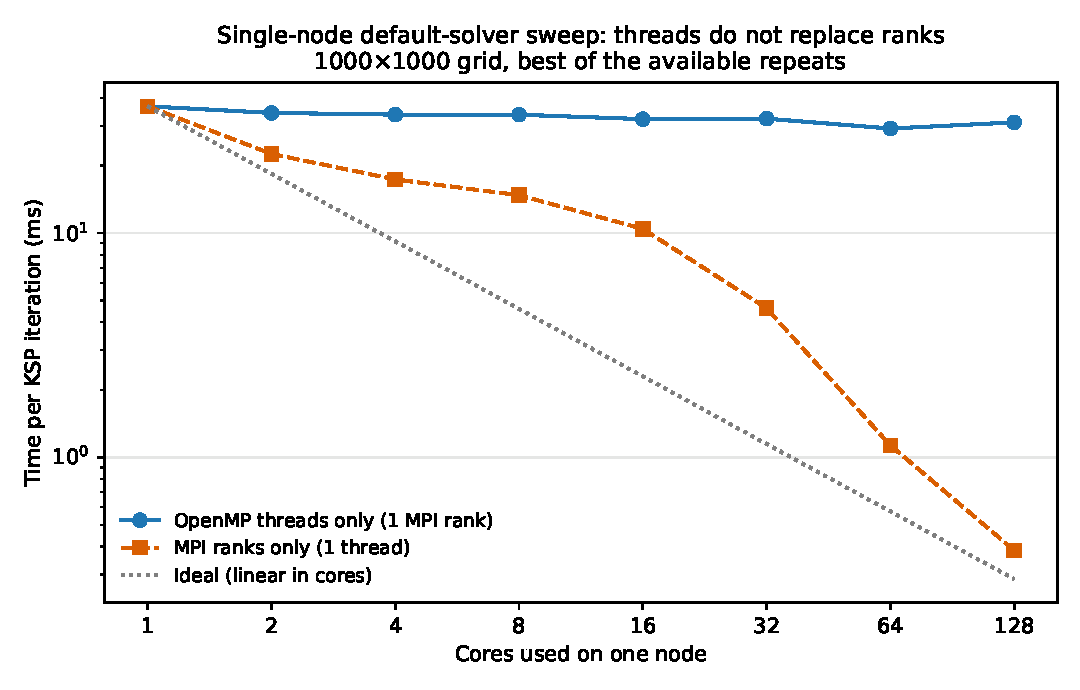
\includegraphics[width=0.85\textwidth]{size_grid_single_node_cost_per_iteration}
  \caption{Single-node default-solver sweep on a $1000\times1000$ grid. Adding OpenMP
  threads to one MPI rank leaves the cost per iteration almost unchanged; adding MPI ranks
  at one thread each reduces it by two orders of magnitude. Both lines start from the same
  one-rank, one-thread run.}
  \label{fig:single-node-sweep}
\end{figure}

Pure OpenMP does not scale. A single rank takes 6700 iterations at every thread count, so
these runtimes are directly comparable, and they barely move: $245.7\,\text{s}$ at one
thread, $225.5$ at eight, $216.5$ at thirty-two, $195.6$ at sixty-four, and $208.4$ at
128. The best case is a factor of 1.26 at 64 threads, after which more threads cost time
again; 128 threads return a factor of 1.18 for 128 times the cores. Over the whole
threads-only line the cost per iteration spans a factor of 1.26; over the ranks-only line
it spans 95.4. The OpenMP backend parallelises only part of the execution path, and the
serial remainder bounds the achievable speedup. \Cref{ch:profiling} returns to this with
profiler evidence.

The MPI-only line from the same baseline reaches $8.1\,\text{s}$ on 64 ranks, a factor of
30. Its rank counts differ, so by \Cref{sec:solver} the wall-clock figure is indicative
rather than a measurement of parallel efficiency; but the 64-rank run performs \emph{more}
iterations than the baseline (7181 against 6700), so iteration count cannot account for
any of the gap. Distributing this problem across the node works, and threading it does not.

Cost per iteration also falls monotonically as ranks replace threads at a fixed core
count, as \Cref{tab:fullnode-cost} shows. Sixteen or more threads per rank is therefore
excluded, and the multi-node study retains 1, 2, 4 and 8.

\begin{table}[ht]
  \centering
  \caption{Cost per KSP iteration for the eight fully populated single-node layouts
  ($\text{ranks}\times\text{threads}=128$) on a $1000\times1000$ grid. The trend is
  monotone in the rank count, with no threshold at any particular thread count. The
  $128\times1$ figure is measured over its non-converged 10,000 iterations, which still
  gives a valid per-iteration cost.}
  \label{tab:fullnode-cost}
  \begin{tabular}{lrrrl}
    \toprule
    Layout & Iterations & Repeats & ms per iteration & Converged \\
    \midrule
    $1\times128$ &  6700 & 1 & 31.10 & yes \\
    $2\times64$  &  3715 & 1 & 14.42 & yes \\
    $4\times32$  &  2825 & 1 &  7.24 & yes \\
    $8\times16$  &  4085 & 1 &  3.67 & yes \\
    $16\times8$  &  8179 & 2 &  1.89 & yes \\
    $32\times4$  &  6460 & 2 &  0.99 & yes \\
    $64\times2$  &  7181 & 2 &  0.61 & yes \\
    $128\times1$ & 10000 & 2 &  0.39 & no \\
    \bottomrule
  \end{tabular}
\end{table}
% VERIFIED 2026-07-31 by analysis/scripts/size_grid/analyze_single_node_sweep.py from the
%   raw logs. Where two repeats exist the values agree to the quoted precision
%   (16x8 1.888-1.893, 32x4 0.9898-0.9910, 64x2 0.6084-0.6092, 128x1 0.3844-0.3866).
%   Table CSV: analysis/data/size_grid/tables/fullnode_cost_per_iteration.csv.
%   NOTE: these are rounded from ms/iteration = Time(sec)/iterations, so they differ in the
%   second decimal from the pre-2026-07-31 prose (14.36/7.20/3.65/1.88/0.98/0.60/0.38),
%   which was read off KSPSolve rather than total Time(sec). Total time is used here for
%   consistency with the wall-clock figures quoted earlier in this section.
% Merged here 2026-07-16 from the dissolved Ch4 "Single-Node Performance Evaluation".
%   Only the per-iteration-safe findings survived; the wall-clock claim that 2-4 threads
%   beat MPI-only was an artefact of block Jacobi block count (see §3.3) and is gone,
%   along with §4.3 "Effect of Solver Choice".
% SOURCE (changed again 2026-07-16, evening): all numbers now come from
%   analysis/data/size_grid/logs/small/*.log (1000x1000 = 1M, arch-omp-opt, jobs 13996330/13997004),
%   because runs/rank_thread_grid/ (the 800² source used briefly) has been DELETED.
%   Same virtues hold: one build, one campaign, and the pure-OpenMP and MPI-only lines
%   share the identical 1-rank/1-thread baseline (245.7 s, 6700 it). Extract from the
%   "Linear solve"/"Time (sec):"/KSPSolve lines in each log. Combos with t<=8 have two
%   reps (both jobids); t>=16 combos have one. Numbers above are from job13996330 rep1.
%   DO NOT pull the MPI-only line from analysis/data/mpi_only/logs/ instead — see G12 below.
% NOTE the honest framing already in the text: this sweep BOUNDS the space, it does not
%   answer which layout is fastest. That question is answered in \Cref{ch:multinode} on
%   CG+GAMG data. Do not let the two get conflated when writing.
% G12 RESOLVED 2026-07-16 (verified from raw logs): analysis/data/mpi_only/logs/ is NOT a separate
%   MPI-only build — all 24 logs are named `arch-mpi-opt` but self-report
%   `on a arch-omp-opt` (label is the job script's, not the binary's). The 1.53x anomaly
%   STANDS, reconstructed indirectly since its direct baseline (rank_thread_grid) is
%   deleted: scaling the size_grid 1M serial run by iteration and size ratios predicts
%   245.7 x (4311/6700) x 0.64 = 101.2 s at 800², matching the deleted 101.3 s baseline;
%   mpi_only measures 154.7 s = 1.53x slower per unit work. Direct same-config check:
%   r128_t1 KSPSolve 2.076 s (mpi_only) vs 1.659 s (fixed128_multinode nodes1) = 1.25x.
%   So the Feb campaign is systematically 1.25-1.5x slower than newer equivalents; cause
%   still unknown (candidates: CPU frequency 3.4/2.25 = 1.51; unbound memory on a remote
%   NUMA node). RULE (relaxed): within-campaign relatives are fine (iteration counts match
%   fixed128_multinode exactly); absolute times need a caveat; cross-campaign absolute
%   comparisons remain off-limits.
% G11 CLOSED, but the MECHANISM for the per-iteration trend is still open. The topology is
%   now measured (\Cref{sec:archer2}) and \Cref{sec:map-matrix} names OpenMP wait time as
%   the cost that grows with threads/rank — but that is a software observation on a
%   different (CG+GAMG, LibSci) campaign. Do NOT retrofit it to this default-solver sweep,
%   and do not assert a NUMA or cache mechanism for either.
% G9 DONE 2026-07-31: \Cref{fig:single-node-sweep}. Both lines are per-iteration rather
%   than speedup, so the MPI-only line's varying iteration count cannot distort it.
% G7 (this section): repetition counts stated in SOURCE note above; when a number goes in
%   the text, cite it as one run or give both reps' spread (e.g. 4x4 ms/it is 9.6-12.0).

\section{Job Configuration and Thread Placement}
\label{sec:placement}
Each rank and its threads are pinned to a contiguous set of cores with:
\begin{verbatim}
OMP_PLACES=cores   OMP_PROC_BIND=close
srun --hint=nomultithread --distribution=block:block --exact
\end{verbatim}

Each part of this is load-bearing, because the whole layout comparison assumes that a
layout means a fixed placement. \texttt{OMP\_PLACES=cores} makes a place one physical
core, so a thread cannot migrate; \texttt{OMP\_PROC\_BIND=close} puts a rank's threads on
adjacent cores rather than spreading them across the node;
\texttt{-{}-hint=nomultithread} uses the 128 physical cores rather than the 256 SMT
siblings; \texttt{-{}-distribution=block:block} gives consecutive ranks consecutive cores,
so ranks that exchange halos are physically adjacent; and \texttt{-{}-exact} restricts a
task to its own \texttt{-{}-cpus-per-task} cores, without which Slurm hands every task the
whole node and the binding is moot. Read against the measured topology of
\Cref{sec:archer2}, close binding on contiguous cores means a $32\times4$ rank occupies
exactly one four-core shared-L3 domain, while a $16\times8$ rank occupies two; no layout
places a rank across two 16-core NUMA regions. Without pinning, threads would migrate
while their first-touched pages stayed put, adding remote memory traffic and run-to-run
variance large enough to swamp the few-per-cent layout effect this study measures.

\section{Metrics}
\label{sec:metrics}
The primary timing is the maximum-rank \texttt{KSPSolve} time in the
\texttt{RepeatedSolves} stage. If this event has count $c=19$, time $t$, and the grid has
$N$ unknowns, steady-state throughput is
\[
  Q = \frac{Nc}{t}.
\]
The analysis also reports $t/(cI)$, where $I$ is the final KSP iteration count. Formal
repeats are aggregated by their median; whiskers show the observed minimum and maximum
from three runs. Scaling is computed per layout against that layout's smallest admitted
node count. For a layout $\ell$ at $n$ nodes,
\[
  S_\ell(n) = \frac{T_\ell(n_0)}{T_\ell(n)}, \qquad
  E_\ell(n) = \frac{S_\ell(n)}{n/n_0},
\]
where $n_0$ is the smallest node count run for that problem size.

\section{Superseded Campaigns}
\label{sec:superseded}
An earlier multi-node campaign covering the same problem sizes and the same four layouts
was collected before the repeated-solve driver existed. It is excluded from every result in
this dissertation, and the reason is decisive: \emph{the layouts it reports were never the
layouts that ran}.

Every PETSc log states the number of MPI processes the library actually initialised, in the
line \texttt{on a <arch> named <node> with <N> process}. Comparing that number against the
rank count encoded in each filename, 141 of the campaign's 142 two-dimensional logs
disagree, and all 161 three-dimensional logs disagree. Most report a single process where
16, 32, 64 or 128 were requested. The job scripts recorded the intended layout in the
filename, but the launcher did not deliver it, so a run labelled $16\times8$ and a run
labelled $128\times1$ may both have executed on one MPI process. Its solve times are 20 to
50 times slower than the corresponding formal runs, which is consistent with that reading.
% VERIFIED 2026-07-31 by comparing the filename rank count against the `with <N> process`
%   header in every non-empty log: ksp_2d_scaling 141/142 mismatch, ksp_3d_scaling 161/161,
%   most reporting N=1. The formal campaigns pass the same check 140/140 in both
%   dimensions. This is the concrete content of the project's "launcher-era" label.
%   CORRECTION: an earlier version of this section attributed the exclusion to the campaign
%   timing single solves and so measuring mostly PCSetUp (median 69% of Time(sec)). That is
%   also true, but it is secondary; no cross-layout quantity from these logs means anything,
%   because the layouts did not take effect.

Any comparison between layouts drawn from those logs is therefore void, including the
conclusion the earlier project material reported, that $32\times4$ is the fastest layout at
every problem size. The apparent ordering reflects how many processes actually started, not
the rank--thread balance.

Two further defects would independently disqualify the campaign. It timed a single solve, so
its reported \texttt{Time (sec)} is dominated by hierarchy construction: \texttt{PCSetUp}
accounts for a median of 69\% of it and is a median of $3.3\times$ the \texttt{KSPSolve}
time. And 72 of its 88 configurations have one recorded run, so no observed range exists.

The experience motivated the validation contract described in \Cref{sec:repro}. Every formal
run in this dissertation is checked against the process and thread counts PETSc itself
reports, and a mismatch fails the pipeline; all 280 formal logs pass. The superseded logs
are retained as provenance (\Cref{app:repo}). The single-node sweep of \Cref{sec:sweep} is a
separate case, unaffected by this defect: its rank counts are confirmed from the logs, and
it is used only for conclusions that hold at a fixed rank count or per iteration.

\section{Reproducibility}
\label{sec:repro}
Every number, table, and figure in \Cref{ch:multinode} and \Cref{ch:profiling} is derived
from raw job output by a script in the accompanying repository, and can be regenerated with
one command per campaign. \Cref{app:repo} lists the layout and the commands.

Three conventions make that possible. First, the raw \texttt{-log\_view} output of every
run is retained unmodified and is the only source of truth; derived CSVs, tables, and
figures are regenerated from it and are never hand-edited. Second, the analysis is
content-validated rather than filename-validated: each parser checks the build that the log
itself reports, the MPI process and OpenMP thread counts PETSc actually saw, the number of
solves and of timed events in the logging stage, and the linked library recorded in the
embedded configure line, and it raises rather than silently dropping a row that fails. A
filename is treated as a label, not as evidence. Third, the claims that the text depends on
are expressed as assertions inside the scripts, so a change in the data that would
invalidate a sentence in this dissertation fails the pipeline instead of passing quietly.
\Cref{tab:iterations-rank} is the clearest case: the script that produces it refuses to
write the table unless the iteration count is constant across thread counts at every fixed
rank count, which is the property \Cref{sec:solver} argues from.

Thirty unit tests cover the parsers and the campaign-completeness checks and run in a
single command. The measured quantities carry the limits stated where they are used: three
repeats support an observed range but not a significance claim, and the exposure shares in
\Cref{sec:bottleneck} are indicators rather than an additive time budget.

The same conventions extend to the profiler evidence. Linaro MAP writes each profile as a
compressed XML document, so the call-tree analysis in \Cref{sec:map-matrix} is produced by
a script that reads the \texttt{.map} files themselves, with no Forge licence and no
export step in the loop. That script validates each profile's layout against the
\texttt{srun} command line recorded inside the file, rejects a profile whose frames MAP
never resolved to libraries, and raises if the ordering the text argues from does not hold.

% ===== Ch4 "Single-Node Performance Evaluation" was DISSOLVED 2026-07-16 =====
%   Decision: merge into Ch3. The single-node sweep is exploratory work that bounds the
%   configuration space, i.e. methodology, not results — and its only two defensible
%   findings (pure OpenMP does not scale; >=16 threads per rank costs more per iteration)
%   now live in \Cref{sec:sweep}. What was cut and why:
%     - "2-4 threads beat MPI-only": artefact of block Jacobi block count (see §3.3).
%     - §4.3 "Effect of Solver Choice": rested on non-converged runs comparing different
%       preconditioners; the defensible argument is now prose in \Cref{sec:solver}.
%   The dissertation is therefore 7 chapters. Chapter numbers renumber automatically;
%   every cross-reference uses \Cref, so nothing else needed changing.
%   On split-back: chapters/ch4_singlenode.tex is now DEAD — delete it, and drop its
%   \include from main.tex.

% ===== FILE: chapters/ch5_multinode.tex =====
\chapter{Full-Node Scaling Results}
\label{ch:multinode}
% Rewritten 2026-07-31 against the audited 2D and 3D repeated-fullnode campaigns,
% re-panelled by unknowns/core band. Invalid launcher-era measurements are excluded.
% §4.7 added 2026-08-01 from the audited fixed-20m strong-scaling campaign (72 logs per
% dimension). Keep it separate from the weak-scaling matrix: different campaign, and the
% 3D 2/4-node anchors sit 0.3-3.1% off the earlier session with no overlapping ranges.
% Claim-to-figure map: ../dissertation_prep/07_claim_evidence_map.md.

\section{Experimental Setup Recap}
\label{sec:mn-setup}
Both corrected campaigns run every node at its full complement of 128 physical cores.
The problem-size filter gives the matched matrix in \Cref{tab:fullnode-matrix}.

\begin{table}[ht]
  \centering
  \caption{Validated repeated-solve matrix. Each dimensionality uses all four layouts
  and three formal repeats at every admitted size--node pair.}
  \label{tab:fullnode-matrix}
  \begin{tabular}{lrrrrl}
    \toprule
    Scale & 2D grid & 2D unknowns & 3D grid & 3D unknowns & Nodes \\
    \midrule
    5m   & $2240^2$  &   5,017,600 & $171^3$ &   5,000,211 & 1 \\
    10m  & $3160^2$  &   9,985,600 & $215^3$ &   9,938,375 & 1, 2 \\
    20m  & $4500^2$  &  20,250,000 & $273^3$ &  20,346,417 & 2, 4 \\
    41m  & $6400^2$  &  40,960,000 & $345^3$ &  41,063,625 & 4, 8 \\
    82m  & $9073^2$  &  82,319,329 & $435^3$ &  82,312,875 & 8, 16 \\
    165m & $12828^2$ & 164,557,584 & $548^3$ & 164,566,592 & 16, 32 \\
    \bottomrule
  \end{tabular}
\end{table}

Each dimensionality contributes 44 formal configurations and 132 formal logs. Eight
earlier 20m pilot logs per dimension are retained as provenance but excluded from every
median and figure. All 280 logs report the intended
\texttt{arch-omp-libsci-rome-opt} build, the requested MPI process and OpenMP thread
counts, and 20 converged solves. The timed stage contains 19 \texttt{KSPSolve} events and
no exact \texttt{PCSetUp}. The embedded PETSc configure record names the threaded
\texttt{libsci\_gnu\_mp.so.5.0} library. The audit found no divergence, PETSc/MPI/Slurm
error, licence wait, or \texttt{CRAYBLAS\_WARNING}. The 140 retrieved 3D source-CSV rows
also match the independently parsed logs one-for-one.

\section{Two Weak-Scaling Chains}
\label{sec:bands}
The admission filter $25{,}000 \leq N/C \leq 100{,}000$ couples problem size to node
count: each scale survives at only one or two node counts, so a panel drawn per problem
size contains two points. The same 11 size--node pairs, however, decompose exactly into
two chains along which the unknowns per core stay near-constant:

\begin{table}[ht]
  \centering
  \caption{The 11 admitted size--node pairs, ordered into two weak-scaling chains.
  Each row holds unknowns per core near-constant while the node count doubles, so a
  layout's cost along a row isolates the effect of concurrency at fixed local work.}
  \label{tab:bands}
  \begin{tabular}{llllllll}
    \toprule
    Band & \multicolumn{6}{c}{Size at node count} & Points \\
    \cmidrule(lr){2-7}
         & 1 & 2 & 4 & 8 & 16 & 32 & \\
    \midrule
    $\sim$40k unknowns/core & 5m & 10m & 20m & 41m & 82m & 165m & 6 \\
    $\sim$80k unknowns/core & 10m & 20m & 41m & 82m & 165m & --- & 5 \\
    \bottomrule
  \end{tabular}
\end{table}

Every admitted configuration falls within 15\% of its nominal band. This dissertation
therefore reports the campaign as weak scaling along these two chains, and treats the
per-size node doublings (\Cref{sec:strong-steps}) as a separate, local observation.
Ideal weak scaling would hold the time per iteration constant along a row; the measured
growth is the cost of concurrency at fixed local work.

\section{2D Results}
\label{sec:2d}
\Cref{fig:2d-throughput} reports steady-state throughput along both chains. Each point is
the median of three formal runs and the whisker spans their observed minimum and maximum.

\begin{figure}[htbp]
  \centering
  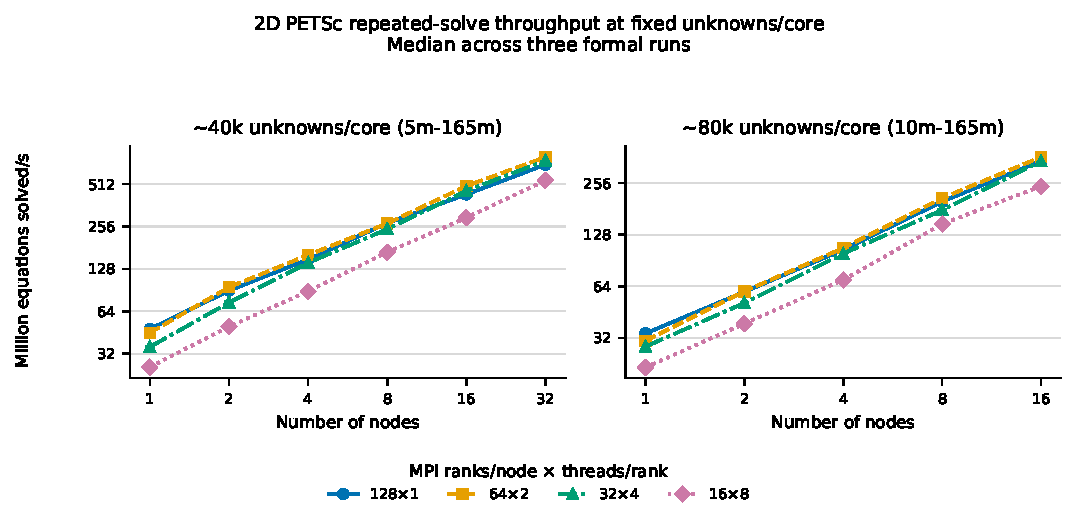
\includegraphics[width=\textwidth]{ksp2d_throughput_vs_nodes}
  \caption{Median 2D repeated-solve throughput along the two unknowns/core chains.
  Whiskers show the observed range of three formal runs. All layouts use 128 cores per
  node, so a fixed node count means a fixed core count.}
  \label{fig:2d-throughput}
\end{figure}

Throughput on a logarithmic axis separates the layouts only weakly, because the dominant
signal is the node count. The comparison that matters is between layouts at a fixed
point, and it is obscured by three orders of magnitude of scale. \Cref{fig:2d-ratio}
therefore divides each layout's time per KSP iteration by that of flat MPI at the same
size--node pair. This normalisation removes both the scale and the 9--13 GAMG iterations,
leaving only the layout effect.

\begin{figure}[htbp]
  \centering
  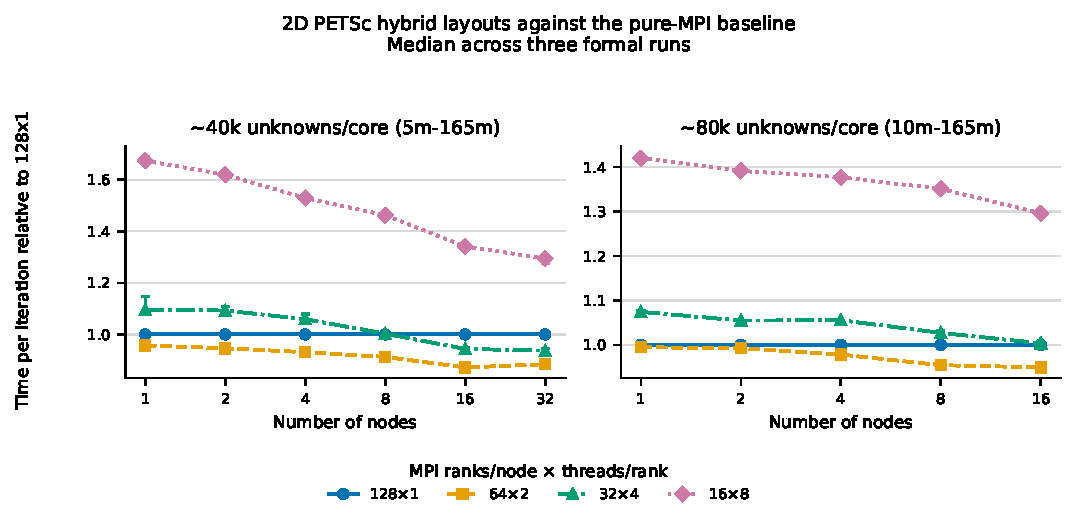
\includegraphics[width=\textwidth]{ksp2d_layout_vs_mpi}
  \caption{2D time per KSP iteration relative to the $128\times1$ baseline at the same
  size--node pair; values below 1 mean the hybrid layout is faster. Whiskers propagate the
  observed range of three formal runs.}
  \label{fig:2d-ratio}
\end{figure}

The result is an ordered trend rather than a set of isolated wins. Along the
$\sim$40k chain, $64\times2$ falls from $0.957$ at one node to $0.872$ at 16 nodes,
$32\times4$ from $1.096$ to $0.937$, and $16\times8$ from $1.674$ to $1.294$. Along the
$\sim$80k chain all three ratios decrease at every step: $64\times2$ from $0.995$ to
$0.949$, $32\times4$ from $1.074$ to $1.004$, and $16\times8$ from $1.420$ to $1.296$.
Four of the six series are strictly monotone, and the two exceptions each contain a single
small reversal ($64\times2$ from $0.872$ to $0.885$ at the last $\sim$40k point, and one
flat step in $32\times4$).

Two consequences follow. First, $64\times2$ is faster than flat MPI per iteration at every
one of the 11 pairs, and its margin widens with concurrency rather than fluctuating.
Second, $32\times4$ is not a fixed loser but a crossing curve: it costs 9.6\% more per
iteration than flat MPI at one node, reaches parity at eight nodes ($1.003$), and is
6.3\% cheaper at 32 nodes. A layout ranking measured at small node counts does not
transfer to large ones.

Raw throughput adds the convergence effect back in and is therefore noisier: $64\times2$
has the highest median at eight of the 11 pairs and flat MPI at the remaining three. Two
of those three flat-MPI wins coincide with flat MPI needing one fewer GAMG iteration; at
the third, 41m on eight nodes, the two medians differ by 0.4\% and their observed ranges
overlap, which is a tie rather than a win. At 164.56 million unknowns on 32 nodes,
$64\times2$ reaches 794.8 million equations per second, 13.1\% above flat MPI; its largest
throughput margin over the matrix is 14.7\%, at 82m on 16 nodes, which is the same point
as its largest per-iteration saving of 12.8\%.

$16\times8$ has the lowest throughput at all 11 pairs and never approaches the baseline,
but the size of its deficit is not constant: it narrows from 46.2\% at 5m on one node to
22.7\% at 165m on 32 nodes.

\section{3D Results}
\label{sec:3d}
The corrected 3D campaign uses the same size--node points, layouts, repeat count, and
measurement contract. The final KSP iteration count ranges from six to seven.

\begin{figure}[htbp]
  \centering
  
\includegraphics[width=\textwidth]{ksp3d_throughput_vs_nodes}
  \caption{Median 3D repeated-solve throughput along the two unknowns/core chains.
  Whiskers show the observed range of three formal runs.}
  \label{fig:3d-throughput}
\end{figure}

\begin{figure}[htbp]
  \centering
  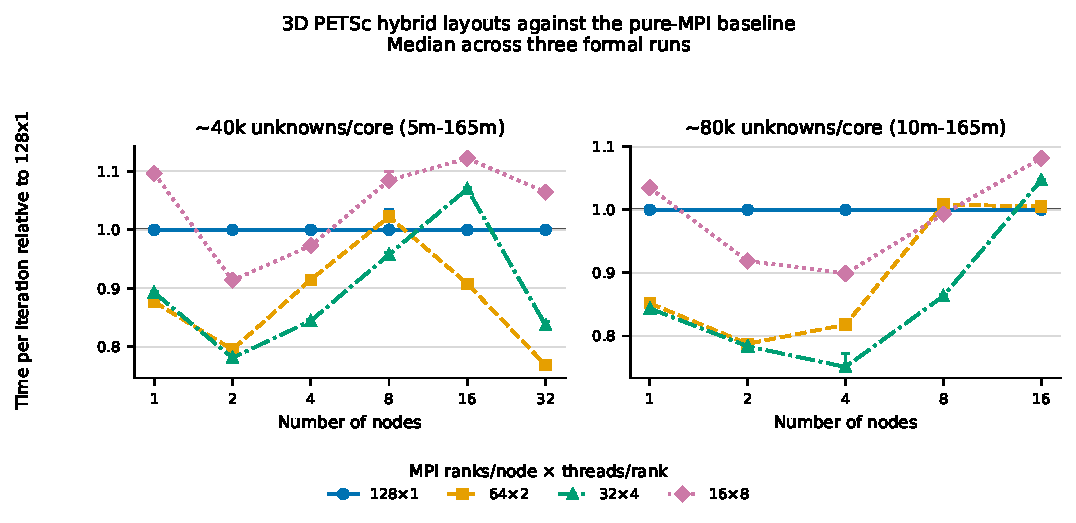
\includegraphics[width=\textwidth]{ksp3d_layout_vs_mpi}
  \caption{3D time per KSP iteration relative to the $128\times1$ baseline at the same
  size--node pair. Unlike the 2D case in \Cref{fig:2d-ratio}, no series is monotone.}
  \label{fig:3d-ratio}
\end{figure}

The 3D behaviour differs from 2D in both magnitude and shape. The advantage is larger: the
best measured point is $32\times4$ at 41m on four nodes, at a ratio of $0.751$, so it
takes 24.9\% less time per iteration than flat MPI where the 2D best takes 12.8\% less.
The same point is the largest raw-throughput margin in either campaign, 33.2\% against a
2D best of 14.7\%; the two pairs of figures differ because a throughput margin is a rate
ratio and a time saving is not. Two-thirds of the 33 hybrid measurements fall below 1,
against 13 of 33 in 2D.
% Both conventions appear in the literature and both appear in this chapter, so they are
%   stated explicitly here once. VERIFIED 2026-08-02 from
%   analysis/data/nproc_2d_libsci/tables/cross_dimension_summary.csv: the maximum time
%   saving and the maximum throughput gain fall at the SAME point in both dimensions
%   (2D 64x2 at 82m/16n, 3D 32x4 at 41m/4n), which is why 12.8/14.7 and 24.9/33.2 pair up.
% VERIFIED 2026-07-31 from repeated_fullnode_formal_summary.csv (both dimensions):
%   ratio<1 counts are 3D 22/33 (64x2 8/11, 32x4 9/11, 16x8 5/11) and 2D 13/33
%   (64x2 11/11, 32x4 2/11, 16x8 0/11).

The advantage is also not ordered by concurrency. Every one of the six series is
non-monotone. Along the $\sim$80k chain the hybrid layouts are strongest at two and four
nodes ($32\times4$ reaching $0.784$ and $0.751$), lose the advantage by eight nodes, and
are at or above parity at 16 nodes, where flat MPI has the lowest time per iteration of
any layout. Along the $\sim$40k chain the pattern recovers at the largest point:
$64\times2$ returns to $0.768$ at 165m on 32 nodes after sitting at $1.022$ at 41m on
eight nodes.

Raw throughput selects $32\times4$ at six of the 11 pairs, $64\times2$ at four, and flat
MPI at one. Iteration-normalised time selects $32\times4$ at seven, $64\times2$ at three,
and flat MPI at one. At 165m on 32 nodes, $64\times2$ reaches 510.4 million equations per
second, 30.1\% above flat MPI. $16\times8$ wins no point, but unlike the 2D case it is not
uniformly the slowest layout: it is faster than flat MPI at five of the 11 pairs.

\section{Weak-Scaling Efficiency}
\label{sec:weak-efficiency}
\Cref{fig:2d-spi} and \Cref{fig:3d-spi} give the absolute time per KSP iteration along
each chain. Ideal weak scaling would be a horizontal line.

\begin{figure}[htbp]
  \centering
  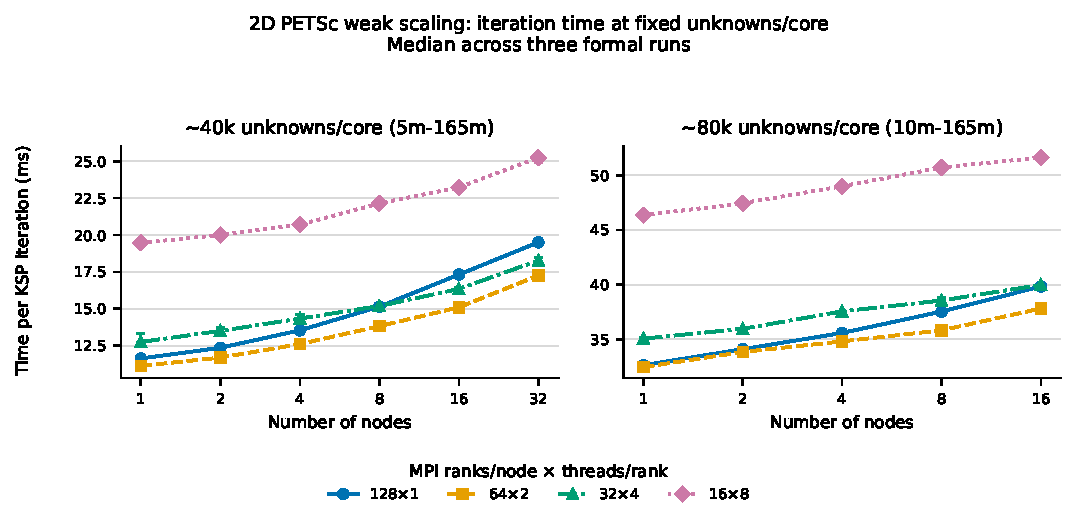
\includegraphics[width=\textwidth]{ksp2d_seconds_per_iteration}
  \caption{Median 2D time per KSP iteration along the two unknowns/core chains. A
  horizontal line would be ideal weak scaling.}
  \label{fig:2d-spi}
\end{figure}

\begin{figure}[htbp]
  \centering
  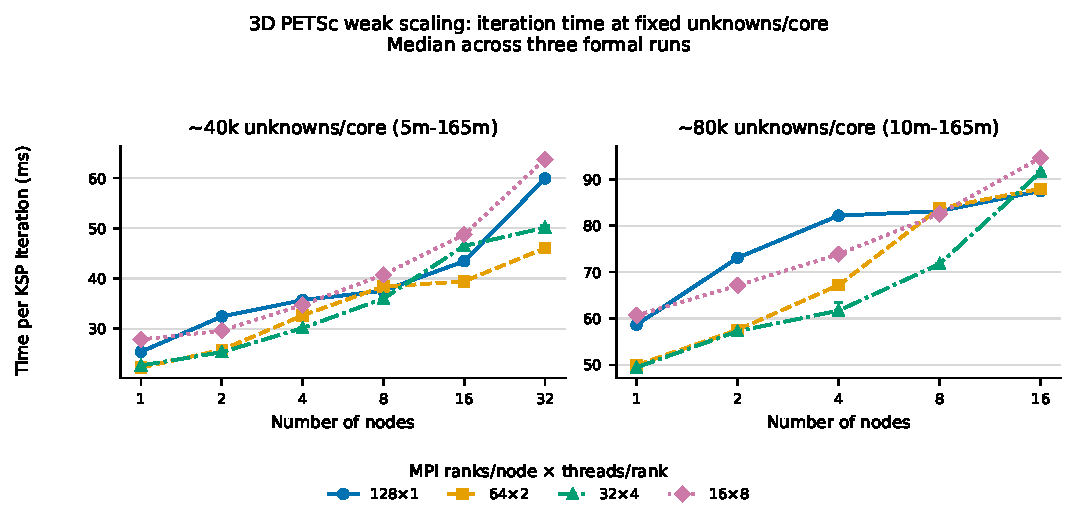
\includegraphics[width=\textwidth]{ksp3d_seconds_per_iteration}
  \caption{Median 3D time per KSP iteration along the two unknowns/core chains.}
  \label{fig:3d-spi}
\end{figure}

Taking each layout's own single-node time as its baseline gives the weak-scaling
efficiencies in \Cref{tab:weak-eff}.

\begin{table}[ht]
  \centering
  \caption{Weak-scaling efficiency (\%) at the largest node count of each chain, relative
  to the same layout's one-node time. Each layout is measured against itself, so this
  quantifies degradation, not absolute speed.}
  \label{tab:weak-eff}
  \begin{tabular}{llrrrr}
    \toprule
    & & \multicolumn{4}{c}{Layout} \\
    \cmidrule(lr){3-6}
    Case & Chain and node count & $128\times1$ & $64\times2$ & $32\times4$ & $16\times8$ \\
    \midrule
    2D & $\sim$40k, 32 nodes & 59.6 & 64.5 & 69.8 & 77.1 \\
    2D & $\sim$80k, 16 nodes & 81.9 & 85.8 & 87.7 & 89.8 \\
    3D & $\sim$40k, 32 nodes & 42.4 & 48.3 & 45.2 & 43.7 \\
    3D & $\sim$80k, 16 nodes & 67.0 & 56.8 & 54.0 & 64.1 \\
    \bottomrule
  \end{tabular}
\end{table}

In 2D the ordering is strict and identical in both chains: efficiency increases with the
number of threads per rank, and $16\times8$ degrades least of all four layouts. This is
consistent with the trend in \Cref{fig:2d-ratio}: replacing MPI ranks with threads reduces
the part of the iteration that grows with node count, which is why the ratio curves fall.
The two metrics measure different things and must not be conflated. $16\times8$ has the
best weak-scaling efficiency and the worst absolute time at every point; it degrades least
because its per-iteration cost is already dominated by a term that does not grow with the
node count. Weak-scaling efficiency measured against a layout's own baseline rewards a
poor baseline.

In 3D no such ordering exists. $64\times2$ degrades least on the $\sim$40k chain, while on
the $\sim$80k chain flat MPI degrades least and both intermediate hybrid layouts degrade
more than either extreme. The 2D mechanism, whatever it is, does not carry over.

\section{Strong-Scaling Steps}
\label{sec:strong-steps}
Five sizes in each dimension have measurements at two adjacent node counts. These are
strong-scaling steps, orthogonal to the weak-scaling chains above, and each size spans one
doubling only. In 2D the four layouts give speedups from 2.00 to 3.08, or apparent
efficiencies from 100.1\% to 154.2\%. The superlinear values are repeatable within this
three-run sample, but the experiment does not identify their cause; cache capacity,
changes in GAMG's distributed hierarchy, and system-level variation all remain possible.
In 3D the range is 1.46 to 2.39, with no superlinear step. At 165m the 16-to-32-node step
gives $1.91\times$ for $64\times2$ against $1.46\times$ for flat MPI.

The largest observed min--max throughput spread among the 44 formal 2D configurations is
4.71\%, and 3.83\% in 3D. Most layout gaps discussed above are larger than that spread,
but three repeats do not support a claim of statistical significance, and the figures
therefore show measured ranges rather than confidence intervals.

\section{Fixed-Size Strong Scaling from One to 32 Nodes}
\label{sec:strong20m}
Single doublings cannot show where a layout stops scaling. A matched extension therefore
holds the problem size fixed and runs the full node sequence $\{1,2,4,8,16,32\}$, giving
six-point strong-scaling curves for every layout in both dimensions. It changes nothing
else: the same \texttt{arch-omp-libsci-rome-opt} build, the same \texttt{ex2\_repeat} and
\texttt{3d\_repeat} drivers, CG with GAMG at \texttt{-ksp\_rtol 1e-5}, one warm-up solve
followed by 19 timed solves in \texttt{RepeatedSolves}, three repeats, 128 cores per node,
and the same four layouts. The fixed problems are $4500^2 = 20{,}250{,}000$ unknowns in 2D
and $273^3 = 20{,}346{,}417$ in 3D, so the two dimensions are matched to within 0.5\%. At
32 nodes this leaves about 4.9 thousand unknowns per core, which is deliberately past the
admission window of \Cref{sec:configspace}: the point is retained as the saturation tail
and should not be read as an efficient operating point.

Each dimension contributes 72 logs, and all 72 passed the same content audit as the formal
matrix. The 2- and 4-node points were rerun as temporal anchors against the corresponding
rows of \Cref{sec:2d} and \Cref{sec:3d}, which were collected in an earlier session. In 2D
the median runtimes differ by at most 2.2\% and six of the eight observed ranges overlap;
in 3D the reruns are 0.3--3.1\% slower and no range overlaps. The 3D offset is small but
systematic, so the two campaigns are reported separately rather than pooled.
% VERIFIED 2026-08-01 from analysis/data/nproc_{2d,3d}_libsci/csv/derived/
%   strong_scaling_20m/strong_scaling_20m_anchor_comparison.csv (8 rows each) and
%   .../strong_scaling_20m_audit.csv (72 rows each, all status=valid).

\begin{figure}[htbp]
  \centering
  
\includegraphics[width=0.85\textwidth]{ksp2d_strong20m_runtime}
  \caption{2D time per solve at a fixed 20.25M unknowns, one to 32 nodes. Both axes are
  logarithmic, so ideal strong scaling is a straight line of slope $-1$. Whiskers show the
  observed range of three formal runs.}
  \label{fig:2d-strong20m}
\end{figure}

\begin{figure}[htbp]
  \centering
  
\includegraphics[width=0.85\textwidth]{ksp3d_strong20m_runtime}
  \caption{3D time per solve at a fixed 20.35M unknowns, one to 32 nodes. Flat MPI and
  $64\times2$ reach a minimum and then get slower, while the two most-threaded layouts
  continue to improve.}
  \label{fig:3d-strong20m}
\end{figure}

The 2D curves in \Cref{fig:2d-strong20m} scale well and stay together. Every layout is
still improving at 32 nodes, and the spread between fastest and slowest widens only from
$1.47\times$ at one node to $1.81\times$ at 16 before narrowing again to $1.48\times$ at
32. $16\times8$ starts 47\% slower than flat MPI and ends 45\% slower, while $64\times2$
and flat MPI end within 2\% of each other. The one-node ordering is also almost the
32-node ordering, differing only by $64\times2$ and flat MPI swapping places: $64\times2$
is fastest at nodes $\{2,4,8,32\}$ and flat MPI at $\{1,16\}$. Cumulative efficiency
exceeds 100\% between two
and 16 nodes, peaking at 191\% for $64\times2$ at eight nodes; as in \Cref{sec:strong-steps}
these superlinear values are repeatable but unexplained by this experiment, and the fixed
problem shrinking into cache is the obvious candidate.

The 3D result in \Cref{fig:3d-strong20m} is qualitatively different, and it is the
strongest layout effect measured anywhere in this study. Every 3D layout eventually stops
scaling and gets \emph{slower}, but they do so at different node counts, and the order is
the thread count. Flat MPI turns first, reaching its minimum at eight nodes, 0.0997\,s per
solve, then 0.1776\,s at 16 and 0.2599\,s at 32. $64\times2$ and $32\times4$ turn one
doubling later, both bottoming at 16 nodes. $16\times8$ has not turned by 32 nodes, where
it is the fastest of the four at 0.0681\,s per solve --- $3.81\times$ faster than flat MPI
on the same 4096 cores, and 10\% faster than $32\times4$, which has already begun to rise.
The observed ranges at that point are disjoint by a wide margin. That the saturation node
count increases monotonically with threads per rank, 8, 16, 16, and beyond 32, is the
clearest single statement this study can make about what hybridisation buys in 3D.
\Cref{tab:strong20m-best} gives the fastest layout at every node count and its margin over
flat MPI.

\begin{table}[ht]
  \centering
  \caption{Fastest full-node layout at each node count for the fixed 20M problems, with
  its median time per solve and its advantage over flat MPI at the same core count.
  Medians of three runs; the 32-node row has about 4.9 thousand unknowns per core.}
  \label{tab:strong20m-best}
  \begin{tabular}{lrlrrlrr}
    \toprule
    & & \multicolumn{3}{c}{2D, $4500^2$} & \multicolumn{3}{c}{3D, $273^3$} \\
    \cmidrule(lr){3-5}\cmidrule(lr){6-8}
    Nodes & Cores & Best & s/solve & vs.\ MPI & Best & s/solve & vs.\ MPI \\
    \midrule
     1 &  128 & $128\times1$ & 0.7704 &  0.0\% & $32\times4$ & 0.8022 &  13.0\% \\
     2 &  256 & $64\times2$  & 0.3365 &  1.0\% & $32\times4$ & 0.4028 &  27.8\% \\
     4 &  512 & $64\times2$  & 0.1265 &  6.9\% & $32\times4$ & 0.2145 &   2.9\% \\
     8 & 1024 & $64\times2$  & 0.0541 &  3.3\% & $64\times2$ & 0.0936 &   6.5\% \\
    16 & 2048 & $128\times1$ & 0.0313 &  0.0\% & $32\times4$ & 0.0652 & 172.4\% \\
    32 & 4096 & $64\times2$  & 0.0277 &  1.9\% & $16\times8$ & 0.0681 & 281.3\% \\
    \bottomrule
  \end{tabular}
\end{table}

\Cref{fig:3d-strong20m-eff} restates the 3D case as parallel efficiency, which is the form
a reader is most likely to have seen for other codes. Each layout is measured against its
own one-node time, so the curves answer "how well does this layout scale?" and not "which
layout is fastest?" --- the two questions have different answers here, and
\Cref{tab:strong20m-endpoints} gives both.

\begin{figure}[htbp]
  \centering
  
\includegraphics[width=0.85\textwidth]{ksp3d_strong20m_efficiency}
  \caption{3D parallel efficiency at a fixed 20.35M unknowns, each layout against its own
  one-node time. Because the baselines differ, this figure ranks scaling behaviour and not
  speed; flat MPI falls to 10.9\% at 32 nodes while $16\times8$ retains 44.5\%.}
  \label{fig:3d-strong20m-eff}
\end{figure}

\Cref{tab:strong20m-endpoints} gives all four layouts at the 32-node endpoint. It also
shows why cumulative efficiency alone would mislead here. In 2D the four layouts reach
almost the same speedup, 27.3 to 29.8, because each is measured against its own one-node
time and $16\times8$ starts from the worst baseline; the runtimes they reach still differ
by 45\%. In 3D the two measures agree, because the layouts diverge rather than converge.

\begin{table}[ht]
  \centering
  \caption{The 32-node endpoint of the fixed-size curves. Speedup and cumulative
  efficiency are measured against the same layout's one-node time, so they reward a poor
  baseline; the doubling efficiency is the 16-to-32-node step alone. Time per solve is the
  only column that compares layouts directly.}
  \label{tab:strong20m-endpoints}
  \begin{tabular}{llrrrr}
    \toprule
    Case & Layout & s/solve & Speedup & Efficiency & 16$\to$32 step \\
    \midrule
    2D & $128\times1$ & 0.0282 & 27.30 & 85.3\% & 55.5\% \\
    2D & $64\times2$  & 0.0277 & 29.83 & 93.2\% & 62.9\% \\
    2D & $32\times4$  & 0.0317 & 27.85 & 87.0\% & 61.1\% \\
    2D & $16\times8$  & 0.0409 & 27.71 & 86.6\% & 69.4\% \\
    \addlinespace
    3D & $128\times1$ & 0.2599 &  3.49 & 10.9\% & 34.2\% \\
    3D & $64\times2$  & 0.1703 &  4.87 & 15.2\% & 22.0\% \\
    3D & $32\times4$  & 0.0747 & 10.75 & 33.6\% & 43.7\% \\
    3D & $16\times8$  & 0.0681 & 14.24 & 44.5\% & 74.6\% \\
    \bottomrule
  \end{tabular}
\end{table}
% VERIFIED 2026-08-01 from analysis/data/nproc_{2d,3d}_libsci/tables/strong_scaling_20m/
%   strong_scaling_20m_{best_layouts,endpoints}.csv, regenerated by
%   analysis/scripts/strong_scaling_20m/analyze_strong_scaling_20m.py.

These runs are noisier than the weak-scaling matrix. The largest observed three-repeat
runtime spread is 10.77\% in 2D, at $32\times4$ on 32 nodes, and 11.09\% in 3D, at
$32\times4$ on eight; the corresponding figures for the formal matrix are 4.71\% and
3.83\%. Both maxima are isolated: the median spread over the 24 configurations is 1.5\% in
2D and 1.0\% in 3D. That is far below
the 3D gaps against flat MPI at 32 and 16 nodes, $3.81\times$ and $2.72\times$, but it is
comparable to the 1--7\% 2D margins over flat MPI, so the 2D ordering at any single node
count should be read as indicative rather than decisive.

Read together with \Cref{sec:2d} and \Cref{sec:3d}, the two regimes answer different
questions and give different answers. At constant work per core the layout effect is
modest and, in 2D, orderly. At constant problem size the effect is unbounded, because the
layouts do not merely differ in speed --- they differ in where they stop scaling. That is
the practical result for a user with a fixed problem and a node-count choice.

\section{Cross-Dimensional Comparison}
\label{sec:cross-dimensional}
The two dimensions differ in the shape of the result, not only in which layout wins.
\Cref{tab:cross-dimension} collects the comparison in one place.

\begin{table}[ht]
  \centering
  \caption{The two dimensions on the quantities this chapter compares them by. The upper
  block is the weak-scaling matrix at constant work per core, the lower block the
  fixed-size curves of \Cref{sec:strong20m}. Throughput gain and time saving are different
  conventions and are both given, because the two dimensions are quoted in both.}
  \label{tab:cross-dimension}
  \begin{tabular}{lll}
    \toprule
    & 2D & 3D \\
    \midrule
    \multicolumn{3}{l}{\emph{Constant work per core, 11 size--node pairs}} \\
    Layout winning most points        & $64\times2$ (8 of 11) & $32\times4$ (6 of 11) \\
    Hybrid points faster per iteration & 13 of 33 & 22 of 33 \\
    Largest throughput gain           & 14.7\% & 33.2\% \\
    Largest per-iteration saving      & 12.8\% & 24.9\% \\
    Ratio series monotone in nodes    & 4 of 6 & 0 of 6 \\
    Weak efficiency rises with threads & yes & no \\
    \addlinespace
    \multicolumn{3}{l}{\emph{Fixed 20M problem, one to 32 nodes}} \\
    Layouts that saturate by 32 nodes & none of 4 & 3 of 4 \\
    First to saturate                 & --- & $128\times1$, at 8 nodes \\
    Fastest at 32 nodes               & $64\times2$ & $16\times8$ \\
    Its lead over flat MPI            & $1.02\times$ & $3.81\times$ \\
    Fastest-to-slowest spread there   & $1.48\times$ & $3.81\times$ \\
    \bottomrule
  \end{tabular}
\end{table}
% VERIFIED 2026-08-02 by analysis/scripts/cross_dimension/summarize_cross_dimension.py ->
%   analysis/data/nproc_2d_libsci/tables/cross_dimension_summary.csv. It joins the two
%   formal summaries, the two strong-scaling summaries and the exposure fits, so no number
%   in this table is transcribed from another chapter by hand.

In 2D the layout effect is ordered and predictable: every hybrid layout improves
relative to flat MPI as concurrency grows, the improvement is monotone along both chains,
$64\times2$ is best everywhere per iteration, and weak-scaling efficiency increases with
threads per rank. In 3D the effect is larger but unordered: the largest throughput margin
is 33.2\% against 14.7\%, yet no series is monotone, the preferred layout changes with
scale and node count, and flat MPI is the least-degrading layout on one of the two chains.
Under strong scaling the asymmetry is sharper still: nothing saturates in 2D within the
measured range, while three of the four 3D layouts do.

The five-point and seven-point stencils perform different work per equation, so their
absolute equations-per-second rates are not direct measures of relative algorithm speed.
The cross-dimensional evidence concerns layout ordering, margins relative to flat MPI, and
the shape of each trend.

\section{Interpretation}
\label{sec:mn-interp}
At constant work per core the measurements place the useful range at two to four threads
per rank in both dimensions. Beyond that the two cases must be stated separately: 2D
supports a single default of $64\times2$ with a margin that grows with concurrency, while
3D supports testing $32\times4$ and $64\times2$ at the target scale, because the ordering
observed at four nodes does not survive to 16.

Eight threads per rank is the one recommendation that depends on the regime. It wins no
point in either weak-scaling campaign and is the slowest 2D layout everywhere, yet
\Cref{sec:strong20m} finds it the fastest 3D layout at 32 nodes on a fixed problem, by a
factor of 3.81 over flat MPI. The two findings are consistent rather than contradictory:
the weak-scaling matrix never drives the work per core below 25 thousand unknowns, which
is where the layouts still resemble each other, and the fixed-size curves continue to
about 4.9 thousand. What eight threads per rank buys is not speed at a comfortable
operating point but a later saturation limit, and it is only worth buying once the
alternatives have stopped scaling.

The 2D trend is consistent with a communication-share explanation: at fixed work per core,
increasing the node count increases the fraction of an iteration spent in halo exchange
and global reduction, and layouts with fewer MPI endpoints pay less of that growth. The
weak-scaling efficiencies in \Cref{tab:weak-eff} order exactly by thread count, which is
what that explanation predicts. \Cref{sec:bottleneck} tests this directly against PETSc's
own event accounting and finds that it holds within each layout, in both dimensions, and
that it also accounts for the non-monotone 3D ordering. What it does not explain is why
$16\times8$ loses everywhere in 2D despite removing the most communication exposure.
\Cref{sec:map-matrix} names that second, countervailing cost from the MAP profiles: time
spent waiting in the OpenMP runtime, which is monotone in the thread count and largest
exactly where $16\times8$ is worst. Those profiles also settle a question the runtime data
could not: the threaded LibSci library that the production build links accounts for at
most 2.1\% of solve-window core-time, so it is not a candidate explanation for anything in
this chapter. What is still missing is a hardware-level account --- why the threads wait
--- and that needs the counter evidence listed in \Cref{sec:futurework}.

% ===== FILE: chapters/ch6_profiling.tex =====
\chapter{Profiling and Bottleneck Analysis}
\label{ch:profiling}
% §6.4 added 2026-07-31: systematic -log_view event analysis over all 264 formal runs.
% §6.3 rewritten 2026-08-01 against the MAP call-tree analysis (11 usable profiles, two
%   builds). Still outstanding: hardware counters to explain WHY the threads wait.
% Fuller draft: ../dissertation_prep/03_draft_profiling_framework.md.

\section{Why a Repeated-Solve Driver}
\label{sec:whyrepeat}
In a single solve at 20.25M with $16\times8$, \texttt{-log\_view} gave \texttt{PCSetUp}
45\% of time and \texttt{KSPSolve} 10\%. \texttt{ex2\_repeat} runs the solve inside a
\texttt{RepeatedSolves} log stage, zeroes the initial guess before each solve, and reuses
the preconditioner (\texttt{-ksp\_reuse\_preconditioner} and
\texttt{-pc\_gamg\_reuse\_interpolation true}). With 20 solves the stage held 69\% of time
and 93\% of flops; within the stage \texttt{KSPSolve} was 100\% of time; each of the 19
repeats took 11 iterations. The corrected scaling campaign uses this same warm-up and
reuse design, so \Cref{ch:multinode} compares steady-state solves rather than first-touch
and hierarchy-construction costs.

\section{Analysis Methodology}
\label{sec:analysis-method}
The method combines MAP 25.0.4 timelines with \texttt{-log\_view} \%T (share of stage
time) and \%F (share of stage flops). An event whose \%T exceeds its \%F spends the
difference on communication, synchronisation, or memory traffic. \Cref{tab:tf} lists
single-point data for the RepeatedSolves stage at 20.25M with $16\times8$.

\begin{table}[ht]
  \centering
  \caption{Per-event time and flop shares, RepeatedSolves stage, 20.25M, $16\times8$.}
  \label{tab:tf}
  \begin{tabular}{lrrr}
    \toprule
    Event & \%T & \%F & GF/s \\
    \midrule
    \texttt{MatMult}          & 39 & 55 & 30.5 \\
    \texttt{MatMultTranspose} & 18 &  6 &  6.7 \\
    \texttt{VecTDot+VecNorm}  &  8 &  6 & --   \\
    \texttt{PCApply} (agg.)   & 82 & 82 & 21.6 \\
    \bottomrule
  \end{tabular}
\end{table}

\texttt{MatMultTranspose} (GAMG restriction) has a \%T three times its \%F and a rate
$4.6\times$ below \texttt{MatMult}. \texttt{VecTDot} and \texttt{VecNorm} are the CG global
reductions.

\section{MAP Profiling Matrix Results}
\label{sec:map-matrix}
Two MAP campaigns profiled the same 20.25M 2D problem: a baseline set on
\texttt{arch-omp-opt} at 2, 8, and 16 nodes, and a matching set on the production
\texttt{arch-omp-libsci-rome-opt} build at 2 and 8 nodes. Neither contains a $128\times1$
cell, because MAP cannot launch 128 MPI ranks per node on this system; flat MPI therefore
has \texttt{-log\_view} evidence only. Of the twelve profiles, eleven are used here. The
16-node $16\times8$ baseline profile is rejected on its own content: MAP resolved no
library symbols in it, so every sample is attributed to its own sampler and the file
carries no cost information.

A \texttt{.map} file is a compressed XML document whose \texttt{sample} elements are
whole-job snapshots of the merged call tree, each node carrying the number of cores active
in that call path. Summing the active cores over the leaves of the tree partitions the
job's core-time by the code that was actually running, which is how MAP itself forms its
percentages, and it can be done from the file alone. The analysis here does that,
validating each profile's layout against the \texttt{srun} line recorded inside the file
rather than against its name, and reports two scopes. The whole-program scope covers every
sample. The solve-window scope keeps only samples in which cores are inside
\texttt{KSPSolve} and none is inside \texttt{PCSetUp}, which approximates the repeated-solve
phase from the profile alone; it is a time window, not the PETSc \texttt{RepeatedSolves}
logging stage, and the two must not be quoted as the same quantity.

\begin{table}[ht]
  \centering
  \caption{Share of total core-time inside the solve window, by the library owning the
  executing frame, for the eleven usable MAP profiles at 20.25M unknowns in 2D. OpenMP is
  the GNU runtime's spin and wait paths, that is threads with no work. MAP instrumentation
  inflates these runs, so the ordering between layouts is the result; the absolute values
  are not transferable to the uninstrumented campaigns.}
  \label{tab:map-shares}
  \begin{tabular}{llrrrrr}
    \toprule
    Build & Nodes & Layout & PETSc & OpenMP & MPI & LibSci \\
    \midrule
    LibSci   &  2 & $64\times2$ & 31.9\% & 36.5\% & 29.9\% & 1.0\% \\
    LibSci   &  2 & $32\times4$ & 51.6\% & 40.1\% &  5.8\% & 1.7\% \\
    LibSci   &  2 & $16\times8$ & 42.2\% & 53.5\% &  1.4\% & 2.1\% \\
    \addlinespace
    LibSci   &  8 & $64\times2$ &  4.5\% & 48.3\% & 46.7\% & 0.2\% \\
    LibSci   &  8 & $32\times4$ &  7.5\% & 69.3\% & 22.6\% & 0.3\% \\
    LibSci   &  8 & $16\times8$ & 15.6\% & 76.5\% &  6.2\% & 1.0\% \\
    \addlinespace
    Baseline &  2 & $32\times4$ & 51.7\% & 40.8\% &  6.7\% & 0.0\% \\
    Baseline &  2 & $16\times8$ & 40.2\% & 57.8\% &  1.4\% & 0.0\% \\
    Baseline &  8 & $32\times4$ &  8.8\% & 68.6\% & 22.2\% & 0.0\% \\
    Baseline &  8 & $16\times8$ & 16.0\% & 77.5\% &  6.0\% & 0.0\% \\
    Baseline & 16 & $32\times4$ &  1.2\% & 69.8\% & 29.0\% & 0.0\% \\
    \bottomrule
  \end{tabular}
\end{table}
% VERIFIED 2026-08-01 by analysis/scripts/map_profiles/analyze_map_profiles.py, which
%   parses the gzipped MAP XML directly (no Forge licence, no `map --export`), validates
%   each profile against its recorded srun line, and RAISES if the solve-window OpenMP
%   share is not increasing in threads/rank or the MPI share not decreasing. Output:
%   analysis/data/nproc_2d_libsci/csv/derived/map_profiles/map_call_tree_shares.csv and
%   .../reports/map_profile_analysis.md. Rows sum to under 100%: libc, the loader and the
%   sampler make up the small "other" remainder, which is omitted from the table.

\begin{figure}[htbp]
  \centering
  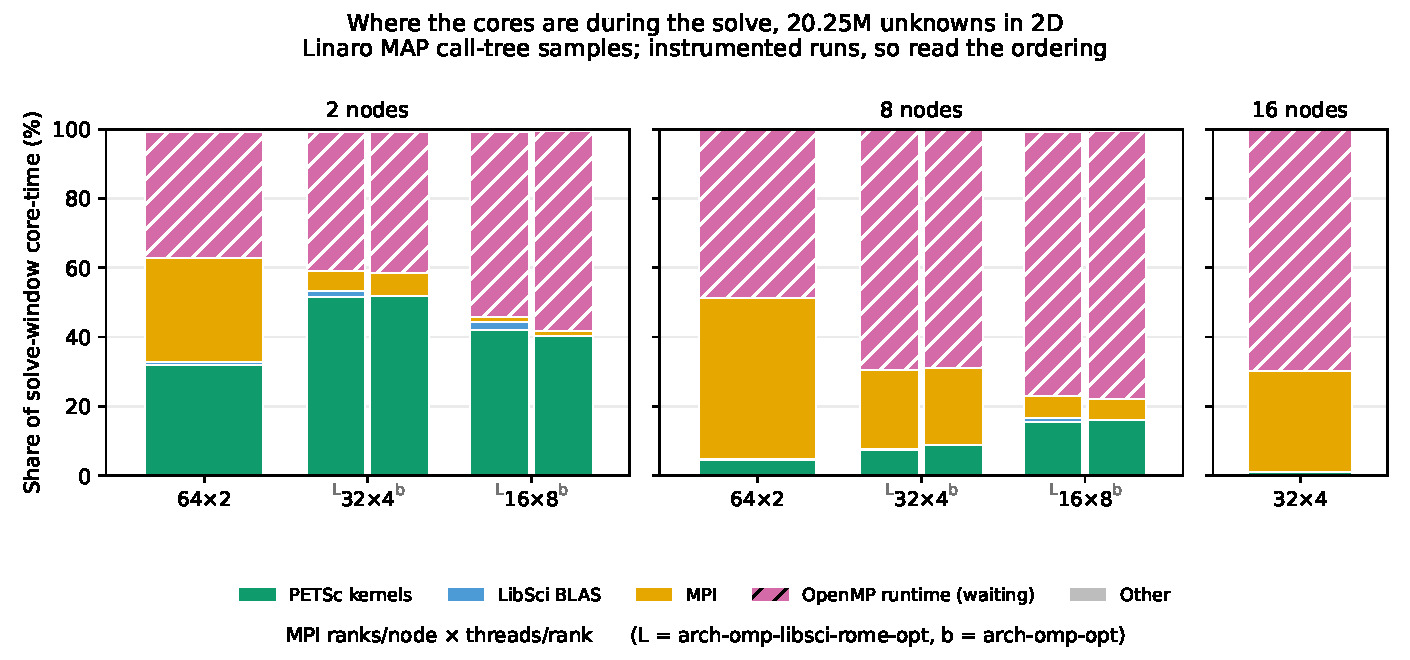
\includegraphics[width=\textwidth]{map_solve_window_shares}
  \caption{Where the cores are during the solve, from the MAP call trees. Within each
  panel the OpenMP waiting share grows and the MPI share shrinks as threads replace ranks,
  and both effects strengthen with node count. Paired bars are the two PETSc builds at the
  same configuration.}
  \label{fig:map-shares}
\end{figure}

\Cref{fig:map-shares} and \Cref{tab:map-shares} name the two costs and show them trading
against each other. The
MPI share falls as threads replace ranks --- at eight nodes it goes 46.7\%, 22.6\%, 6.2\%
across $64\times2$, $32\times4$, $16\times8$ --- which is the same ordering that
\Cref{sec:bottleneck} obtains from \texttt{-log\_view} on the whole formal matrix, here
reproduced by a different instrument on a different quantity. The time spent in the OpenMP
runtime runs the other way, 48.3\%, 69.3\%, 76.5\%, and it is not useful work: the frames
are \texttt{cpu\_relax}, \texttt{do\_spin} and \texttt{\_\_futex\_wait}, that is threads
waiting for something to do. The two builds agree wherever they overlap: across the four
common cells the MPI shares differ by at most 0.9 percentage points and the OpenMP shares
by at most 4.3, with no systematic sign. This is a property of the layout, not of the
linked library.

Three limits apply. MAP's overhead is large and uneven --- separately measured at $+35\%$
on the timed stage and roughly threefold on \texttt{VecScatterEnd} --- and its OpenMP
instrumentation perturbs exactly the barrier behaviour being measured, so the absolute
percentages overstate what an uninstrumented run would show. There is one profile per
cell, so there is no observed range. And with no $128\times1$ profile the trend is
anchored only at its hybrid end, though flat MPI has no OpenMP runtime time at all by
construction, which fixes the missing point at zero.

Within those limits the table answers the question \Cref{ch:multinode} left open. The
cost that grows with threads per rank, and that must be repaid before hybridisation
helps, is idle time in the OpenMP runtime, not NUMA placement and not L3 capacity. It has
the right shape: it is monotone in the thread count, it grows with node count as the work
per threaded region shrinks, and it is largest exactly where $16\times8$ performs worst.
\Cref{sec:bottleneck} shows the other half of the trade, on the full matrix and without a
profiler.

A fourth observation is negative and worth recording. Threaded LibSci is linked into the
production build and PETSc's sparse solve path barely calls it: BLAS accounts for at most
2.1\% of solve-window core-time in any LibSci profile, and the baseline profiles sample no
BLAS frame at all. The threaded BLAS library therefore cannot account for the layout
ordering measured in \Cref{ch:multinode}, which confirms from profile data what
\Cref{sec:threats} could previously only state as a limit of the evidence.

\section{Bottleneck Identification}
\label{sec:bottleneck}
\Cref{sec:map-matrix} leaves the hardware question open, but the \texttt{-log\_view} event
tables of the uninstrumented formal runs support a narrower question that
\Cref{ch:multinode} raised and could not answer: whether the layout effect tracks the share
of the solve exposed to inter-process synchronisation. All 264 formal runs are parsed here,
so the evidence covers the same matrix as the scaling results and carries no profiler
overhead.

\subsection*{What is measured}
For each run, the time of the halo-exchange events (\texttt{VecScatterBegin},
\texttt{VecScatterEnd}) and of CG's global-reduction events (\texttt{VecTDot},
\texttt{VecNorm}) is taken from the \texttt{RepeatedSolves} stage and divided by that
stage's \texttt{KSPSolve} time. Three limits apply and none is removable from
\texttt{-log\_view} alone. The synchronising events are logged \emph{inside}
\texttt{MatMult} and its relatives, so this is an exposure share and not a term in an
additive time budget; summing every leaf event against \texttt{KSPSolve} gives 116--372\%.
Each event time is a maximum over ranks, and different events may attain their maximum on
different ranks. \texttt{VecTDot} and \texttt{VecNorm} also perform local flops, so their
time is not purely communication. The quantity is nevertheless measured identically in
every run, which is what makes it comparable across layouts and node counts.
% VERIFIED 2026-07-31 by analysis/scripts/nproc_2d_libsci/analyze_event_breakdown.py.
%   It also asserts that SFPack/SFUnpack have call counts identical to
%   VecScatterBegin/End (they are nested inside them) and excludes them, because
%   counting both double-counts the halo exchange by roughly a third.

\subsection*{Halo exchange dominates, and hybridisation reduces it}
\Cref{fig:2d-sync} and \Cref{fig:3d-sync} give the result. In both dimensions the share
rises monotonically with node count for every layout, and at 21 of the 22 size--node points
it is strictly ordered by MPI rank count: fewer ranks, less exposure. Halo exchange is the
larger term throughout. In 2D at 165m on 32 nodes it accounts for 34.3 of flat MPI's 48.2
percentage points, against 13.9 for the reductions; in 3D at the same point it accounts for
70.9 of 84.6. The 3D shares are far higher than the 2D shares at every comparable point,
which is consistent with the seven-point stencil's larger surface-to-volume ratio.

\begin{figure}[htbp]
  \centering
  
\includegraphics[width=0.85\textwidth]{ksp2d_sync_share}
  \caption{2D share of \texttt{RepeatedSolves} \texttt{KSPSolve} time spent inside halo
  exchange and global reduction events. The ordering matches the time-per-iteration
  ordering in \Cref{fig:2d-ratio} at every node count.}
  \label{fig:2d-sync}
\end{figure}

\begin{figure}[htbp]
  \centering
  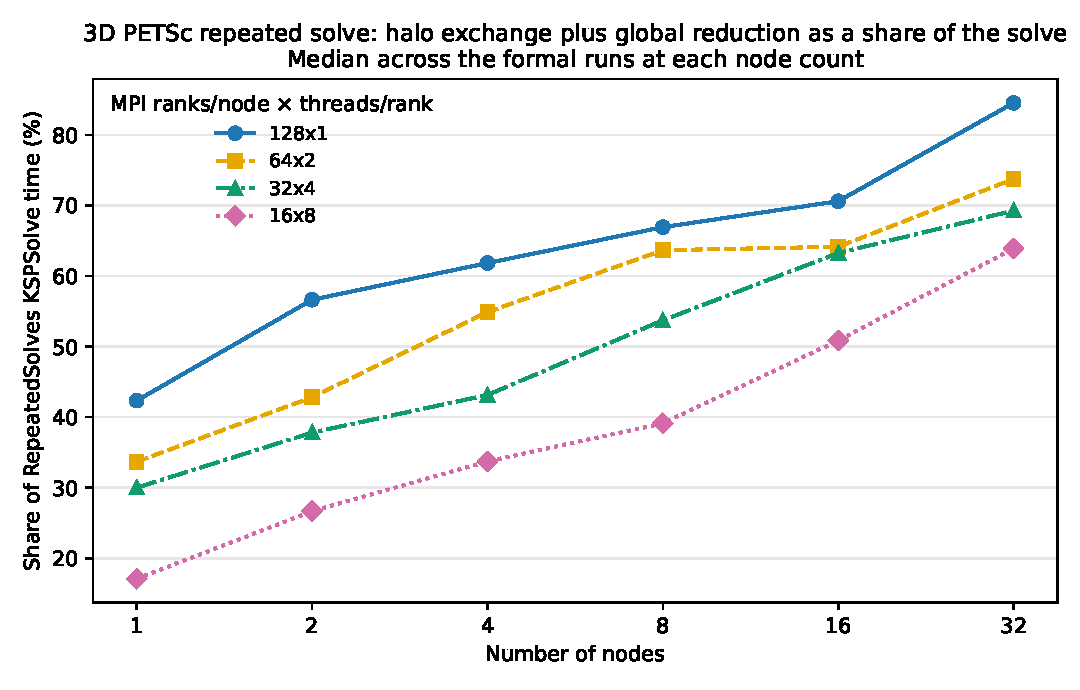
\includegraphics[width=0.85\textwidth]{ksp3d_sync_share}
  \caption{3D share of \texttt{RepeatedSolves} \texttt{KSPSolve} time spent inside halo
  exchange and global reduction events. Note the vertical scale: flat MPI reaches 84.6\%
  at the largest point.}
  \label{fig:3d-sync}
\end{figure}

\subsection*{Reduced exposure is necessary but not sufficient}
The ordering alone cannot explain the results, because $16\times8$ has the lowest exposure
at nearly every point and the worst time per iteration at all 11 points in 2D. What does
track performance is the \emph{size} of the reduction. Within a single layout, comparing
its exposure against flat MPI at the same size--node point with its time per iteration
relative to flat MPI gives the fits in \Cref{tab:sync-breakeven}.

\begin{table}[ht]
  \centering
  \caption{Reduction in synchronisation exposure relative to flat MPI at the same
  size--node point, against time per iteration relative to flat MPI. The break-even column
  is where the fitted line crosses parity, i.e. how much exposure a layout must remove
  before its thread overhead is repaid. Eleven points per layout; the fits are descriptive.}
  \label{tab:sync-breakeven}
  \begin{tabular}{llrrrr}
    \toprule
    Case & Layout & Exposure removed (pt) & Time ratio & $r$ & Break-even (pt) \\
    \midrule
    2D & $64\times2$ &  0.8--7.4  & 0.872--0.995 & $-0.67$ & 1.2 \\
    2D & $32\times4$ &  5.3--13.7 & 0.937--1.096 & $-0.59$ & 11.7 \\
    2D & $16\times8$ &  6.3--21.9 & 1.294--1.674 & $+0.00$ & not reached \\
    3D & $64\times2$ &  1.9--15.1 & 0.768--1.022 & $-0.86$ & 2.9 \\
    3D & $32\times4$ &  5.5--23.5 & 0.751--1.070 & $-0.90$ & 7.3 \\
    3D & $16\times8$ & 17.4--31.1 & 0.899--1.122 & $-0.83$ & 26.7 \\
    \bottomrule
  \end{tabular}
\end{table}

\Cref{fig:3d-tradeoff} plots the 3D case that the table summarises. The three layouts form
three roughly parallel descending lines, displaced from each other along the horizontal
axis: each removes more exposure than the one before it, and each needs more of it before
crossing parity.

\begin{figure}[htbp]
  \centering
  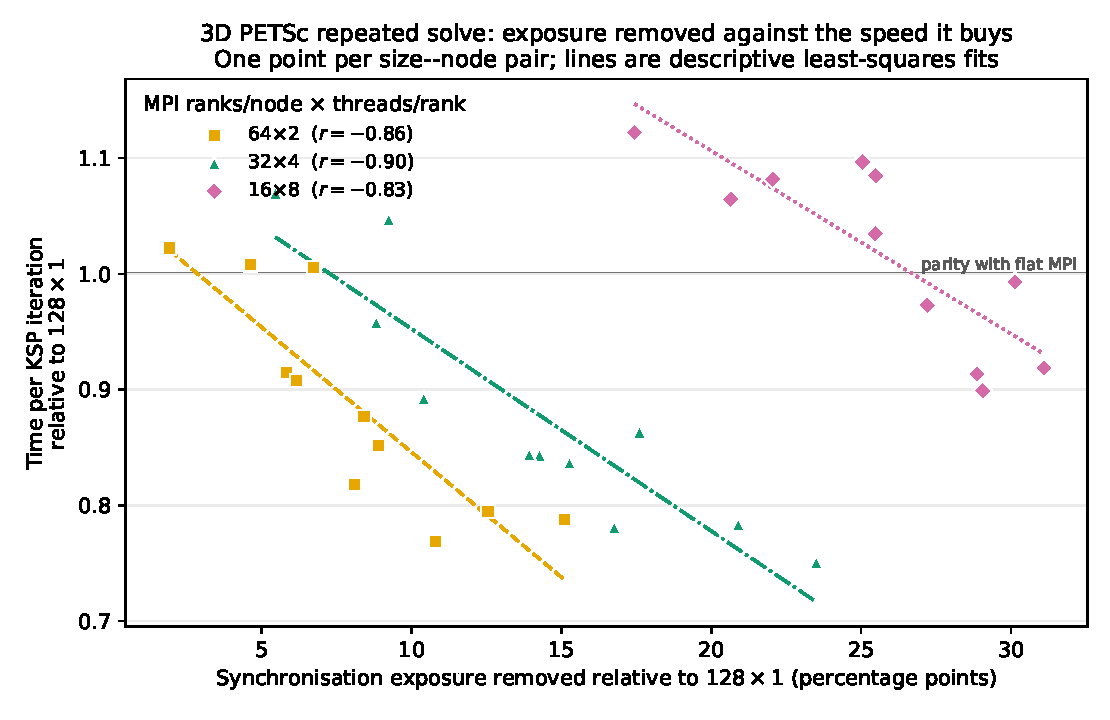
\includegraphics[width=0.85\textwidth]{ksp3d_exposure_tradeoff}
  \caption{3D exposure removed relative to flat MPI against the resulting time per
  iteration, one point per size--node pair. Where a layout's fitted line crosses parity is
  the break-even column of \Cref{tab:sync-breakeven}; the lines are descriptive, not
  predictive.}
  \label{fig:3d-tradeoff}
\end{figure}

Five of the six correlations are negative and three exceed $0.8$ in magnitude: the more
exposure a layout removes at a given point, the faster it is relative to flat MPI there.
The break-even column quantifies the trade-off that \Cref{ch:multinode} could only assert.
Each doubling of threads per rank removes more exposure but demands more before it pays:
1.2, then 11.7, then unreachable in 2D; 2.9, then 7.3, then 26.7 in 3D. No break-even
figure is an extrapolation --- every one of them, where it exists, falls inside the range
of exposure the layout was actually observed to remove.

This explains the two things Ch5 could not. In 3D at 41m on four nodes, $32\times4$ removes
23.5 points and is the fastest measured configuration at $0.751$; four nodes later at 41m
on eight nodes, $64\times2$ removes only 2.0 points and loses at $1.022$. The 3D advantage
is non-monotone because the exposure it removes is non-monotone, not because the mechanism
differs. In 2D, $32\times4$ crosses parity between eight and 16 nodes precisely as its
removed exposure passes its 11.7-point break-even: 9.6 points at 41m on eight nodes for a
ratio of 1.003, and 13.7 points at 82m on 16 nodes for 0.944.

The 2D $16\times8$ row is the honest counter-example, and \Cref{fig:2d-tradeoff} shows it
as a flat cloud among two descending lines. Its correlation is zero: exposure removal
predicts nothing there, because the layout is slower than flat MPI by 29--67\% at every
point and some other cost dominates entirely.

\begin{figure}[htbp]
  \centering
  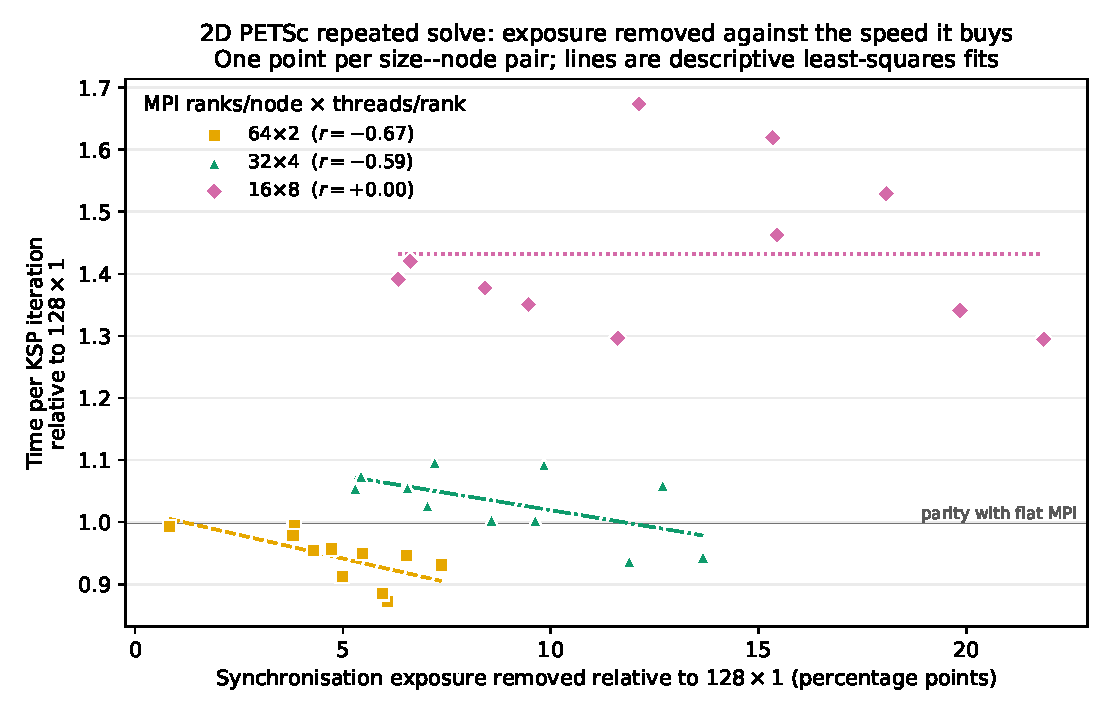
\includegraphics[width=0.85\textwidth]{ksp2d_exposure_tradeoff}
  \caption{2D exposure removed relative to flat MPI against the resulting time per
  iteration. Compare with \Cref{fig:3d-tradeoff}: $64\times2$ and $32\times4$ descend as
  they do in 3D, but $16\times8$ sits well above parity at every point with no slope at
  all.}
  \label{fig:2d-tradeoff}
\end{figure}
 \Cref{tab:map-shares} identifies that
cost: at the same problem size and node counts, $16\times8$ spends more of its core-time
waiting in the OpenMP runtime than any other layout, 76.5\% against 48.3\% for
$64\times2$ at eight nodes. The two halves of the trade are therefore both measured, one
on the full matrix without a profiler and the other on eleven profiled cells with one.
What remains unmeasured is their sum: the profiled and unprofiled quantities come from
different instruments on different runs and cannot be added into a single budget.

\subsection*{What this does and does not establish}
Pooling all 33 hybrid measurements per dimension inverts the sign of the correlation
($-0.58$ in 2D), because $16\times8$ combines the largest exposure reduction with the worst
performance. The relationship is therefore a within-layout one, and reporting a pooled
figure would be misleading.

These data identify \emph{where} the layout advantage comes from within PETSc's own event
accounting: reduced exposure to halo exchange, with global reduction second and much less
layout-sensitive. Together with \Cref{sec:map-matrix} they locate the countervailing cost
in the OpenMP runtime rather than at a memory boundary. Neither identifies a
\emph{hardware} mechanism. The exposure share cannot separate message latency, bandwidth,
rank-count-dependent metadata, and waiting caused by load imbalance elsewhere in the
iteration; and knowing that threads wait does not say whether they wait because PETSc
threads only part of the path, because the threaded regions are too short to amortise a
barrier, or because memory bandwidth is already saturated. Separating those, and
attributing anything to cache capacity, needs the hardware-counter work listed in
\Cref{sec:futurework}.

% G8 CLOSED 2026-07-31: the placeholder section "Preconditioner Reuse in the Scaling
%   Context" is REMOVED. Its intended content is already stated where it is load-bearing:
%   the motivation and the 69%/93% stage shares in \Cref{sec:whyrepeat}, the reuse options
%   and the zeroed initial guess in \Cref{sec:benchmarks}, and the scope limit it implies
%   ("applies to applications that solve repeatedly with the same operator") in
%   \Cref{sec:threats}. A separate section would only repeat them.

% ===== FILE: chapters/ch7_discussion.tex =====
\chapter{Discussion}
\label{ch:discussion}
% Write once results are final. Outline: 00 §Ch7.

\section{Answering the Research Questions}
\label{sec:rqs}
Hybrid execution reduces steady-state solve time in both dimensions, but the two cases
answer the question differently, and the difference is in the shape of the result rather
than in which layout happens to win.

In 2D the answer is ordered. Along both unknowns/core chains, every hybrid layout improves
relative to flat MPI as the node count grows, and the improvement is monotone in four of
the six measured series. $64\times2$ has a lower time per iteration than flat MPI at all
11 size--node points, and its margin widens from 4.3\% at one node to 12.8\% at 16 nodes.
$32\times4$ crosses from 9.6\% slower at one node to 6.3\% faster at 32. A layout
comparison performed at small node counts therefore does not transfer to large ones,
which is the practical content of the 2D result.

In 3D the effect is larger but unordered. The best hybrid margin is 33.2\%, against 14.7\%
in 2D, and two-thirds of the hybrid measurements are faster than flat MPI. No series is
monotone: the advantage peaks at two to four nodes, disappears by eight to 16, and returns
at the largest point. Raw throughput selects $32\times4$ at six of 11 points, $64\times2$
at four, and flat MPI at one. The preferred balance depends on problem size and node count
in a way that the 2D data do not.

Held at a fixed problem size instead, the same question has a much larger answer. On
20.25M unknowns in 2D the four layouts stay within a factor of 1.81 of each other from one
to 32 nodes and all are still scaling at the end. On the matched 20.35M 3D problem they
diverge:
every layout eventually saturates, but the node count at which it does rises with the
thread count --- eight nodes for flat MPI, 16 for $64\times2$ and $32\times4$, beyond 32
for $16\times8$. Flat MPI is $2.6\times$ slower at 32 nodes than at its own optimum, so the
gap to $16\times8$ at 4096 cores reaches $3.81\times$. The strong-scaling regime does not
change which layouts are good at moderate scale, but it changes the stakes from
single-digit percentages to factors, because what differs between layouts is where they
stop scaling.

$16\times8$ wins no raw-throughput point in either weak-scaling campaign, yet it has the
best weak-scaling efficiency of all four layouts in 2D. The two statements are compatible:
weak-scaling efficiency measures a layout against its own baseline, and $16\times8$
degrades least because its per-iteration cost is already dominated by a term that does not
grow with concurrency. On its own that is a caution about the metric rather than a
recommendation. The fixed-size curves of \Cref{sec:strong20m} turn it into one for a
specific case: driven past the admission window to about 4.9 thousand unknowns per core,
$16\times8$ is the fastest 3D layout at 32 nodes, $3.81\times$ faster than flat MPI, which
by then has been getting slower for two doublings, and the only layout of the four that
has not yet saturated. Eight threads per rank buys a later saturation limit, not a better
operating point.

That contrast is the clearest methodological result of the study. The same eleven
size--node pairs, read at constant work per core, place the useful range at two to four
threads and rank $16\times8$ last; the same solver and build on a fixed problem make
$16\times8$ the only 3D layout still improving at 4096 cores. A layout recommendation is
meaningless without the scaling regime it was measured in.

Raw throughput includes changes in GAMG convergence, whereas time per iteration controls
for the outer KSP count. The normalised metric does not make the GAMG hierarchy or
communication volume identical across decompositions. Both views are needed: raw
throughput measures the time paid by this solver configuration, while time per iteration
separates the clearest convergence-count effect.

On where the time goes, the answer is now partly positive. \Cref{sec:bottleneck} shows that
hybridisation reduces the share of the solve exposed to halo exchange and global reduction
at 21 of the 22 size--node points, that halo exchange is the larger term throughout, and
that within each layout the size of that reduction correlates with how much faster the
layout is than flat MPI ($|r|$ up to $0.90$). Each doubling of threads per rank removes more
exposure but must remove more before it pays, which is why the useful range is two to four
threads and why the 3D ordering is non-monotone.

The second half of that trade is measured too, on eleven Linaro MAP profiles of the 20.25M
2D problem. Within the solve window the share of core-time spent waiting in the OpenMP
runtime rises with threads per rank --- 48.3\%, 69.3\%, 76.5\% at eight nodes --- while the
MPI share falls, 46.7\%, 22.6\%, 6.2\%. Both orderings reproduce across two different
PETSc builds. This names the cost that repays hybridisation as OpenMP idle time rather than
NUMA placement or L3 capacity, and it explains why $16\times8$ removes the most exposure
in 2D and is still the slowest layout at every point.

What remains unexplained is one level lower. Knowing that threads wait does not say why:
partial threading of PETSc's solve path, threaded regions too short to amortise a barrier,
and saturated memory bandwidth all predict the same signature, and the exposure share
likewise cannot separate message latency, bandwidth, rank-count-dependent metadata, and
imbalance elsewhere in the iteration. The profiled and unprofiled quantities also come
from different instruments and cannot be summed into one time budget. No hardware
mechanism is established here.

\section{Threats to Validity}
\label{sec:threats}
The validated matrix covers two structured-grid Poisson problems, one PETSc version and
compiler environment, and one CG+GAMG configuration. The conclusions need not transfer
to unstructured matrices, other preconditioners, or solver phases that call dense BLAS.
Preconditioner reuse removes setup from the timed stage, so the result applies to
applications that solve repeatedly with the same operator rather than end-to-end single
solves. That scope limit is not incidental: as \Cref{sec:superseded} shows, a campaign that
timed single solves instead ranked the layouts differently, because setup accounted for a
median of 69\% of its measured time. An application dominated by one-off solves should
expect the setup ranking, not the one reported here.

Three repeats quantify the observed range but are insufficient for strong significance
claims or a detailed noise model. Within the formal matrix the unknowns-per-core filter
gives at most two node counts per problem size, so every strong-scaling step there covers
one doubling. Reading the same points as two weak-scaling chains recovers six- and
five-point curves, but does not add measurements: the chains and the doublings describe
one campaign of 11 size--node pairs, and a trend seen along a chain is supported by those
points alone. The fixed-size extension of \Cref{sec:strong20m} supplies genuine six-point
curves, but at one problem size per dimension; whether the 3D saturation ordering holds at
other sizes is untested, and its 32-node point sits outside the admission window by
design. Its three-repeat spreads are also larger, up to 11.1\%, because the per-solve time
at the largest node counts is only a few tens of milliseconds.

Weak-scaling efficiency is computed against each layout's own single-node time, so it
measures degradation and not speed, and it rewards a layout whose baseline is poor. It
must be read together with \Cref{fig:2d-ratio} and \Cref{fig:3d-ratio}, never on its own.

Iteration normalisation controls the 9--13 iterations in 2D and 6--7 in 3D, but not
decomposition-dependent GAMG work within an iteration. The single-node configuration-space
study used the default rank-dependent block-Jacobi solver and provides boundary evidence
rather than production layout rankings. It is further limited by a defect established in
\Cref{sec:solver}: its job script's double-dashed \texttt{-{}-ksp\_rtol 1e-5} was never
consumed by PETSc, so those runs converged against a mesh-dependent tolerance that
tightens as $1/N$, reaching $2.4\times10^{-10}$ at $6400^2$. The exploratory campaigns
therefore differ from the production ones in both solver and tolerance, and no
default-versus-GAMG performance comparison is drawn from them. The conclusions that do
rest on that sweep hold at a fixed rank count or per iteration, where the tolerance is
common to the runs being compared. All formal runs pass the option with a single dash.

The formal runs used a binary linked to threaded LibSci. \Cref{sec:map-matrix} now shows
directly that the repeated sparse solve barely calls it, at most 2.1\% of solve-window
core-time, so LibSci is excluded as an explanation rather than merely unproven as one.
MAP timings remain excluded from the scaling curves because profiler overhead is large and
uneven, and for the same reason the profile shares are read as an ordering between layouts
and not as absolute costs; there is one profile per cell and none at $128\times1$.
Hardware-mechanism claims remain outside the evidence established here.

\section{Practical Guidance for PETSc on ARCHER2}
\label{sec:guidance}
For this repeated 2D CG+GAMG workload, $64\times2$ is the best default among the tested
full-node layouts, and the case for it strengthens with job size: it is faster per
iteration than flat MPI at every measured point, by 4.3\% at one node and 12.8\% at 16.
Small one-node jobs should still test flat MPI, which gives 5.9\% and 9.5\% higher raw
throughput than $64\times2$ at 5m and 10m because it converges in one fewer GAMG
iteration. Jobs above roughly eight nodes should also test $32\times4$, which is slower
than flat MPI below that point and faster above it.

For the matched 3D workload, test both $32\times4$ and $64\times2$ at the intended node
count, and do not extrapolate from a smaller one. $32\times4$ wins more points across the
matrix and gives the single largest margin, 33.2\% at 41m on four nodes, but $64\times2$
is the better choice at 165m on 32 nodes, where it exceeds flat MPI by 30.1\%. On the
$\sim$80k chain at 16 nodes no hybrid layout beats flat MPI at all.

The $16\times8$ layout wins no raw-throughput point in either dimension at constant work
per core, so eight threads per rank should not be a default. Its favourable weak-scaling
efficiency in 2D is not evidence for it, for the reason given in \Cref{sec:threats}. There
is one case where it should be tried: a fixed 3D problem pushed to the point where the
other layouts have stopped scaling. At about 5 thousand unknowns per core on 32 nodes it
was the fastest layout measured and the only one still improving, while flat MPI had been
getting slower for two doublings and both intermediate layouts for one.

The general form of that advice is worth stating separately, because it is the guidance
most likely to be applied wrongly. Choose the layout for the regime the job actually runs
in. If the work per core is comfortable --- above roughly 25 thousand unknowns --- the
layouts differ by single-digit percentages and $64\times2$ is a safe default in 2D, with
$32\times4$ worth testing in 3D. If instead the problem is fixed and the node count is
being pushed for time to solution, the choice is worth factors, and it is the most-threaded
layouts that keep scaling. A benchmark run at one node, or at comfortable occupancy, does
not answer the second question.

% ===== FILE: chapters/ch8_conclusion.tex =====
\chapter{Conclusion and Future Work}
\label{ch:conclusion}

\section{Conclusions}
\label{sec:conclusions}
The corrected 2D and 3D campaigns contain 264 formal runs across 88 configurations from
one to 32 ARCHER2 nodes, and the matched fixed-size extension adds 144 more across 48
configurations. Sixteen pilot logs are preserved but excluded from the statistics. Every
formal run uses one warm-up solve and 19 timed solves with the GAMG hierarchy reused, and
every one was validated against the build, layout, convergence and library that PETSc
itself reports.

At constant work per core, moderate hybridisation provides the most reliable range in both
dimensions and eight threads per rank is not competitive in either. Beyond that, the two
cases differ in kind.

The 2D layout effect is ordered by concurrency. Read as weak scaling at fixed
unknowns/core, every hybrid layout improves relative to flat MPI as the node count grows,
monotonically in four of the six measured series. $64\times2$ is faster per iteration than
flat MPI at all 11 size--node points, by 4.3\% at one node and 12.8\% at 16, and at
164.56M unknowns on 32 nodes it reaches 794.8 million equations per second, 13.1\% above
flat MPI on raw throughput. $32\times4$ crosses from 9.6\% slower at one node to 6.3\%
faster at 32.

The 3D effect is larger but unordered. The best margin is 33.2\%, at 41m on four nodes,
and two-thirds of the hybrid measurements beat flat MPI, but no series is monotone and the
preferred layout changes with scale and node count. At the matched largest point,
$64\times2$ reaches 510.4 million equations per second, 30.1\% above flat MPI, while one
node later on the other chain no hybrid layout wins at all.

Held at a fixed problem size instead of fixed work per core, the same layouts separate far
more sharply. Over one to 32 nodes the 2D curves stay within a factor of 1.81 of each
other and all four are still improving at 4096 cores. The matched 3D curves diverge,
because each layout saturates and turns upward at a node count that rises with its thread
count: eight nodes for flat MPI, which is $2.6\times$ slower again by 32; 16 nodes for
$64\times2$ and $32\times4$; and beyond 32 for $16\times8$, which is last in every
weak-scaling comparison and yet the fastest layout at 32 nodes, by a factor of 3.81 over
flat MPI. What distinguishes the layouts under strong scaling is not their speed but where
they stop scaling, so a layout recommendation without its scaling regime is not a
recommendation.

Profiling locates both sides of the trade. PETSc's own event data show hybridisation
reducing exposure to halo exchange and global reduction, and eleven Linaro MAP profiles
show the cost that must be repaid: within the solve window the share of core-time spent
waiting in the OpenMP runtime rises with threads per rank, 48.3\% to 76.5\% at eight nodes,
reproducibly across two PETSc builds. The same profiles rule out the linked threaded BLAS
library as an explanation, at most 2.1\% of solve-window core-time.

These measurements replace the invalid launcher-era layout rankings. They support
$64\times2$ as the default for repeated 2D CG+GAMG solves, with the margin growing rather
than shrinking at scale; a $32\times4$ versus $64\times2$ comparison performed at the
target node count in 3D; and the most-threaded layouts where a fixed problem is pushed
past the point at which the others saturate. Flat MPI remains competitive for small 2D
jobs and for selected 3D decompositions. The current evidence establishes these
performance patterns and names the software cost behind them, but not the hardware
mechanism underneath it.

\section{Future Work}
\label{sec:futurework}
The MAP profiles establish that the threads wait; hardware counters are needed to
establish why. Memory-bandwidth and cache-miss counters, taken per layout at a fixed
size and node count, would separate the three candidate causes that the profiles cannot:
PETSc threading only part of the solve path, threaded regions too short to amortise an
OpenMP barrier, and bandwidth saturation before all cores are busy. Instrumenting PETSc's
threaded regions directly, rather than sampling them, would give the first of those
without a counter at all.

The profiled matrix is also thin. It covers one problem size, two node counts on the
production build, three hybrid layouts, and one run per cell, and MAP cannot produce the
flat-MPI cell that would anchor the trend. Repeating it at a second size, and at the node
counts where the 3D fixed-size curves turn upward, would test whether the OpenMP wait
share predicts the saturation point rather than merely accompanying it.

Two extensions follow from the fixed-size results. A second and third fixed problem size
would show whether the 3D saturation ordering is a property of the layouts or of 20M
unknowns, and node counts beyond 32 would locate the turning point of $32\times4$ and
$16\times8$, which this campaign brackets only from below. More repeats at close layout
pairs would support confidence intervals in place of min--max ranges. Further experiments
should include preconditioner setup, changing operators, unstructured matrices, other
compiler environments, and GPU execution.

%============================================================ back matter
\printbibliography[heading=bibintoc]

\appendix

% ===== FILE: chapters/appendix.tex =====
\chapter{Reproducibility: Repository and Scripts}
\label{app:repo}
The repository accompanying this dissertation contains the benchmark sources, the ARCHER2
job scripts, every raw log, and the analysis pipeline that turns one into the other.

\section{Layout}
\label{app:layout}

\begin{table}[ht]
  \centering
  \caption{Repository layout. Raw logs and retrieved job CSVs are immutable evidence;
  everything under a \emph{derived} heading is regenerated by the scripts.}
  \label{tab:repo-layout}
  \begin{tabular}{ll}
    \toprule
    Path & Contents \\
    \midrule
    \texttt{src/} & Benchmark drivers (\Cref{sec:benchmarks}) \\
    \texttt{scripts/ksp/\{2d,3d\}/lib/} & Slurm job scripts and problem-size tables \\
    \texttt{scripts/petsc\_configure\_archer2.sh} & PETSc configure recipes for both builds \\
    \addlinespace
    \texttt{analysis/data/<campaign>/logs/} & Raw \texttt{-log\_view} output, immutable \\
    \texttt{analysis/data/<campaign>/csv/source/} & Retrieved job CSVs, byte-for-byte \\
    \texttt{analysis/maps/<campaign>/} & Linaro MAP profiles, immutable \\
    \texttt{analysis/data/<campaign>/csv/derived/} & Derived: normalised and aggregated CSVs \\
    \texttt{analysis/data/<campaign>/tables/} & Derived: reference tables \\
    \texttt{analysis/plots/<campaign>/} & Derived: figures, as PNG and PDF pairs \\
    \texttt{analysis/scripts/<campaign>/} & Analysis code and its unit tests \\
    \addlinespace
    \texttt{docs/dissertation\_latex/} & This document and \texttt{sync\_figures.sh} \\
    \bottomrule
  \end{tabular}
\end{table}

The campaigns are named for the study that produced them. The results in this dissertation
come from \texttt{nproc\_2d\_libsci} and \texttt{nproc\_3d\_libsci}, which hold both the
validated repeated-solve matrices and, under \texttt{strong\_scaling\_20m}, the fixed-size
extension of \Cref{sec:strong20m}; \texttt{size\_grid} holds the single-node
configuration-space sweep of \Cref{sec:sweep}, and \texttt{profiling\_2d\_map\_baseline}
the baseline MAP profiles of \Cref{sec:map-matrix}. The earlier \texttt{ksp\_2d\_scaling},
\texttt{ksp\_3d\_scaling}, \texttt{mpi\_only} and \texttt{fixed128\_multinode} campaigns
are retained as provenance and are not used for any layout claim, for the reasons given in
\Cref{sec:solver} and \Cref{sec:threats}.

\section{Evidence Index}
\label{app:evidence}
Every numbered figure and table in this dissertation is derived from raw job output by one
of six scripts. \Cref{tab:evidence-index} gives the chain for each: which script produced
it, which derived file that script writes, and which raw evidence the script consumed. To
check any number, run the script named in its row and compare; to check the number's
provenance instead, read the raw evidence directly, which is retained unmodified.

\begin{table}[ht]
  \centering
  \caption{Evidence index. Script paths are relative to
  \texttt{analysis/scripts/}, derived and raw paths to \texttt{analysis/}. Log
  counts are the files present, which for the 3D fixed-size campaign exceeds the 72
  accepted runs because superseded job attempts are retained. The last two rows are read
  directly from a named file and have no derived stage.}
  \label{tab:evidence-index}
  \footnotesize
  \begin{tabular}{L{0.155\textwidth} L{0.215\textwidth} L{0.245\textwidth} L{0.235\textwidth}}
    \toprule
    Figures and tables & Generated by & Derived output & Raw evidence \\
    \midrule
    \Cref{tab:iterations-rank}, \Cref{tab:fullnode-cost}, \Cref{fig:single-node-sweep}
      & \texttt{size\_grid/ analyze\_single\_node\_ sweep.py}
      & \texttt{data/size\_grid/tables/ iterations\_vs\_ layout.csv}, \texttt{fullnode\_cost\_per\_ iteration.csv}
      & \texttt{data/size\_grid/logs/} \newline 213 logs \\
    \addlinespace
    \Cref{tab:fullnode-matrix}, \Cref{tab:weak-eff}, \Cref{fig:2d-throughput}--\Cref{fig:3d-spi}
      & \texttt{nproc\_\{2d,3d\}\_libsci/ analyze\_repeated\_ fullnode\_logs.py}
      & \texttt{csv/derived/repeated\_ fullnode\_formal\_ summary.csv}
      & \texttt{logs/repeated\_ fullnode/} \newline 140 logs per dimension \\
    \addlinespace
    \Cref{tab:strong20m-best}, \Cref{tab:strong20m-endpoints}, \Cref{fig:2d-strong20m}--\Cref{fig:3d-strong20m-eff}
      & \texttt{strong\_scaling\_20m/ analyze\_strong\_ scaling\_20m.py}
      & \texttt{csv/derived/strong\_ scaling\_20m/*.csv}, \texttt{tables/strong\_ scaling\_20m/*.csv}
      & \texttt{logs/strong\_ scaling\_20m/} \newline 72 (2D) and 108 (3D) logs \\
    \addlinespace
    \Cref{tab:cross-dimension}
      & \texttt{cross\_dimension/ summarize\_cross\_ dimension.py}
      & \texttt{tables/cross\_dimension\_ summary.csv}
      & joins the three rows above \\
    \addlinespace
    \Cref{tab:map-shares}, \Cref{fig:map-shares}
      & \texttt{map\_profiles/ analyze\_map\_ profiles.py}
      & \texttt{csv/derived/map\_ profiles/map\_call\_tree\_ shares.csv}
      & \texttt{maps/} \newline 12 MAP profiles, 11 usable \\
    \addlinespace
    \Cref{tab:sync-breakeven}, \Cref{fig:2d-sync}--\Cref{fig:2d-tradeoff}
      & \texttt{nproc\_2d\_libsci/ analyze\_event\_ breakdown.py} \newline (covers both dimensions)
      & \texttt{tables/repeated\_ fullnode\_event\_ matrix.csv}, \texttt{repeated\_fullnode\_ exposure\_fits.csv}
      & \texttt{logs/repeated\_ fullnode/} \newline as above \\
    \addlinespace
    \Cref{tab:layouts}, \Cref{tab:rtol}
      & read directly
      & ---
      & \texttt{scripts/ksp/ diagnostics/ petsc\_diagnostics. 14598711.out} \\
    \addlinespace
    \Cref{tab:cg-ops}, \Cref{tab:tf}
      & read directly
      & ---
      & one named \texttt{-log\_view} log each, cited in place \\
    \bottomrule
  \end{tabular}
\end{table}

\Cref{tab:models} and \Cref{tab:bands} state definitions rather than measurements and have
no evidence chain: the first classifies the execution models and the second restates the
admission rule of \Cref{sec:configspace}. \Cref{fig:archer2_architecture} is reproduced
from the ARCHER2 hardware documentation.

\section{Regenerating the results}
\label{app:regen}
From the repository root, after creating the analysis environment with
\texttt{python3 -m venv analysis/.venv} and
\texttt{analysis/.venv/bin/pip install -r requirements.txt}:

\begin{verbatim}
# unit tests (30)
analysis/.venv/bin/python -m pytest -c analysis/pytest.ini analysis/scripts

# single-node configuration-space sweep  -> Table 3.2, Table 3.3, Figure 3.1
analysis/.venv/bin/python \
    analysis/scripts/size_grid/analyze_single_node_sweep.py

# 2D and 3D repeated-solve campaigns     -> Chapter 4 weak-scaling figures
analysis/.venv/bin/python \
    analysis/scripts/nproc_2d_libsci/analyze_repeated_fullnode_logs.py
analysis/.venv/bin/python \
    analysis/scripts/nproc_3d_libsci/analyze_repeated_fullnode_logs.py

# matched fixed-20m strong scaling       -> Section 4.7
analysis/.venv/bin/python \
    analysis/scripts/strong_scaling_20m/analyze_strong_scaling_20m.py \
    --dimension 2d
analysis/.venv/bin/python \
    analysis/scripts/strong_scaling_20m/analyze_strong_scaling_20m.py \
    --dimension 3d

# event-level breakdown and exposure fits -> Section 5.4
analysis/.venv/bin/python \
    analysis/scripts/nproc_2d_libsci/analyze_event_breakdown.py

# Linaro MAP call-tree shares            -> Section 5.3
analysis/.venv/bin/python \
    analysis/scripts/map_profiles/analyze_map_profiles.py

# cross-dimensional comparison           -> Table 4.6
analysis/.venv/bin/python \
    analysis/scripts/cross_dimension/summarize_cross_dimension.py

# copy the generated PDFs into this document's figures/ directory
bash docs/dissertation_latex/sync_figures.sh
\end{verbatim}

Each script prints the number of logs it validated and the configurations it aggregated,
and exits non-zero if any check fails. The document is then built with
\texttt{tectonic docs/dissertation\_latex/draft.tex}.

\chapter{Full log\_view Excerpts}
\label{app:logs}
% Optional: before/after RepeatedSolves log_view listings referenced in Ch6.

\end{document}
